\documentclass{article}
\usepackage[utf8]{inputenc}
\usepackage[margin=1in]{geometry}
\usepackage{graphicx}
\usepackage{amsmath,amscd}
\usepackage{amssymb}
\usepackage{amsthm}
\usepackage{mathptmx}

\begin{document}
\title{Summary of Heuristic-based Kinematics of Containment, 2D case}
\maketitle

\begin{enumerate}
\item {\bf General settings}\\
Let ${\bf a}=[a_1, a_2]^T$ denotes the semi-axis of the smaller ellipse $E_a$, and so the semi-axis of bigger ellipse $E_b$ can be defined as ${\bf b}=[b_1,b_2]^T=(1+\epsilon){\bf a}$, where $\epsilon$ is the ``explode factor''. We further define the aspect ratio of the ellipses as $\alpha = a_1/a_2 = b_1/b_2$. Therefore, there are only 3 parameters to be considered in this problem, say ``$a_2, \alpha, \epsilon$''.

\item {\bf Largest angle that the smaller ellipse can rotate}\\
The maximum angle that the smaller ellipse can rotate comes when the center point is fixed in the origin. And the angle can be found in closed-form as follows.

We use the parametric forms for the two ellipses,
\begin{equation}
\begin{aligned}
{\bf u}_a = \left( 
\begin{aligned}
a_1 \cos \theta_a\\
a_2 \cos \theta_a
\end{aligned}
\right) &&
{\bf u}_b = \left( 
\begin{aligned}
b_1 \cos \theta_b\\
b_2 \cos \theta_b
\end{aligned}
\right)
\end{aligned}
\end{equation}

and the rotation of $E_a$ can be written as,
\begin{equation}
R(\phi) = \left(
\begin{aligned}
\cos\phi && -\sin\phi\\
\sin\phi && \cos\phi
\end{aligned}\right)
\end{equation}
where $\phi$ is the rotational angle of $E_a$.

Assume that the bigger ellipse $E_b$ is fixed with the world frame, with the center in the origin, and the larger semi-axis is aligned with x-axis. Then the points on the boundary of $E_b$ as seen in the world frame is exactly ${\bf u}_b$. Since $E_a$ only rotates around the origin, the points on its boundary as seen in the world frame should be $R(\phi) {\bf u}_a$.

The intersecting point of the two ellipses can be obtained by enforcing the two parametric equations as seen in the world frame to be equal as,
\begin{equation}
\begin{aligned}
& {\bf u}_b = R(\phi) {\bf u}_a \\
\iff & \left\{
\begin{aligned}
b_1 \cos\theta_b = a_1\cos\phi \cos\theta_a - a_2\sin\phi \sin\theta_a\\
b_2 \sin\theta_b = a_1\sin\phi \cos\theta_a + a_2\cos\phi \sin\theta_a
\end{aligned}
\right.\\
\end{aligned}
\end{equation}
Substituting $a_1 = \alpha a_2, b_1 = (1+\epsilon)a_1, b_2 = (1+\epsilon)a_2$, and observing the fact that $\theta_b = \phi + \theta_a$ (rotational angle transformation from local frame to world frame of $E_a$) gives,
\begin{equation}
\begin{aligned}
& \left\{
\begin{aligned}
\alpha a_2 (1+\epsilon) \cos(\theta_a + \phi) = \alpha a_2 \cos\phi \cos\theta_a - a_2\sin\phi \sin\theta_a\\
a_2 (1+\epsilon) \sin(\theta_a + \phi) = \alpha a_2 \sin\phi \cos\theta_a + a_2\cos\phi \sin\theta_a
\end{aligned}
\right. \\
\iff & 
\left\{
\begin{aligned}
\alpha \epsilon \cos\theta_a \cos\phi = (\alpha(1+\epsilon) - 1) \sin\theta_a \sin\phi \\
\epsilon \sin\theta_a \cos\phi = (\alpha - \epsilon - 1) \cos\theta_a \sin\phi \\
\end{aligned}
\right. \\
\end{aligned}
\end{equation}
Since always $a_2 < b_2$, the points on smaller semi-axis of the smaller ellipse will be always inside the bigger ellipse, so when we consider the case of intersecting, $\theta_a \neq \pi/2$, or $3\pi/2$, or $\cos\theta_a \neq 0$. Further, One sufficient condition when two ellipses intersect should be $a_1 \geq b_2$, or $\alpha \geq 1+\epsilon$, and the equal sign occurs only when $\phi = \pi/2, 3\pi/2$ and $\theta_a = 0, \pi$, or $\cos\phi = 0$ and $\sin\theta_a = 0$.

So, for general cases, we could rearrange the above system of equations as,
\begin{equation}
\left\{
\begin{aligned}
\frac{\alpha \epsilon}{(\alpha(1+\epsilon)-1)} = \tan\theta_a \tan\phi \\
\frac{\epsilon}{(\alpha - \epsilon - 1)} \tan\theta_a = \tan\phi
\end{aligned}
\right.
\end{equation}
Since $b_1 \geq a_1$, $\phi \neq 0, \pi$ ($\tan\phi \neq 0$) when two ellipses intersect, then we could get,
\begin{equation}
\begin{aligned}
& \frac{\alpha \epsilon}{(\alpha(1+\epsilon)-1) \tan\phi} = \frac{(\alpha - \epsilon - 1) \tan\phi}{\epsilon}\\
\Rightarrow & \tan^2\phi = \frac{\alpha \epsilon^2}{(\alpha(1+\epsilon)-1)(\alpha - \epsilon - 1)}
\end{aligned}
\end{equation}
Solving for $\phi$ gives,
\begin{equation}
\phi = \arctan (\pm \epsilon \sqrt[]{\frac{\alpha}{(\alpha(1+\epsilon)-1)(\alpha - \epsilon - 1)}})
\end{equation}

Figures \ref{diff-alpha} and \ref{diff-epi} show the numerical experiments to verify the result, with different $\alpha$ and $\epsilon$ values respectively.

\begin{figure}
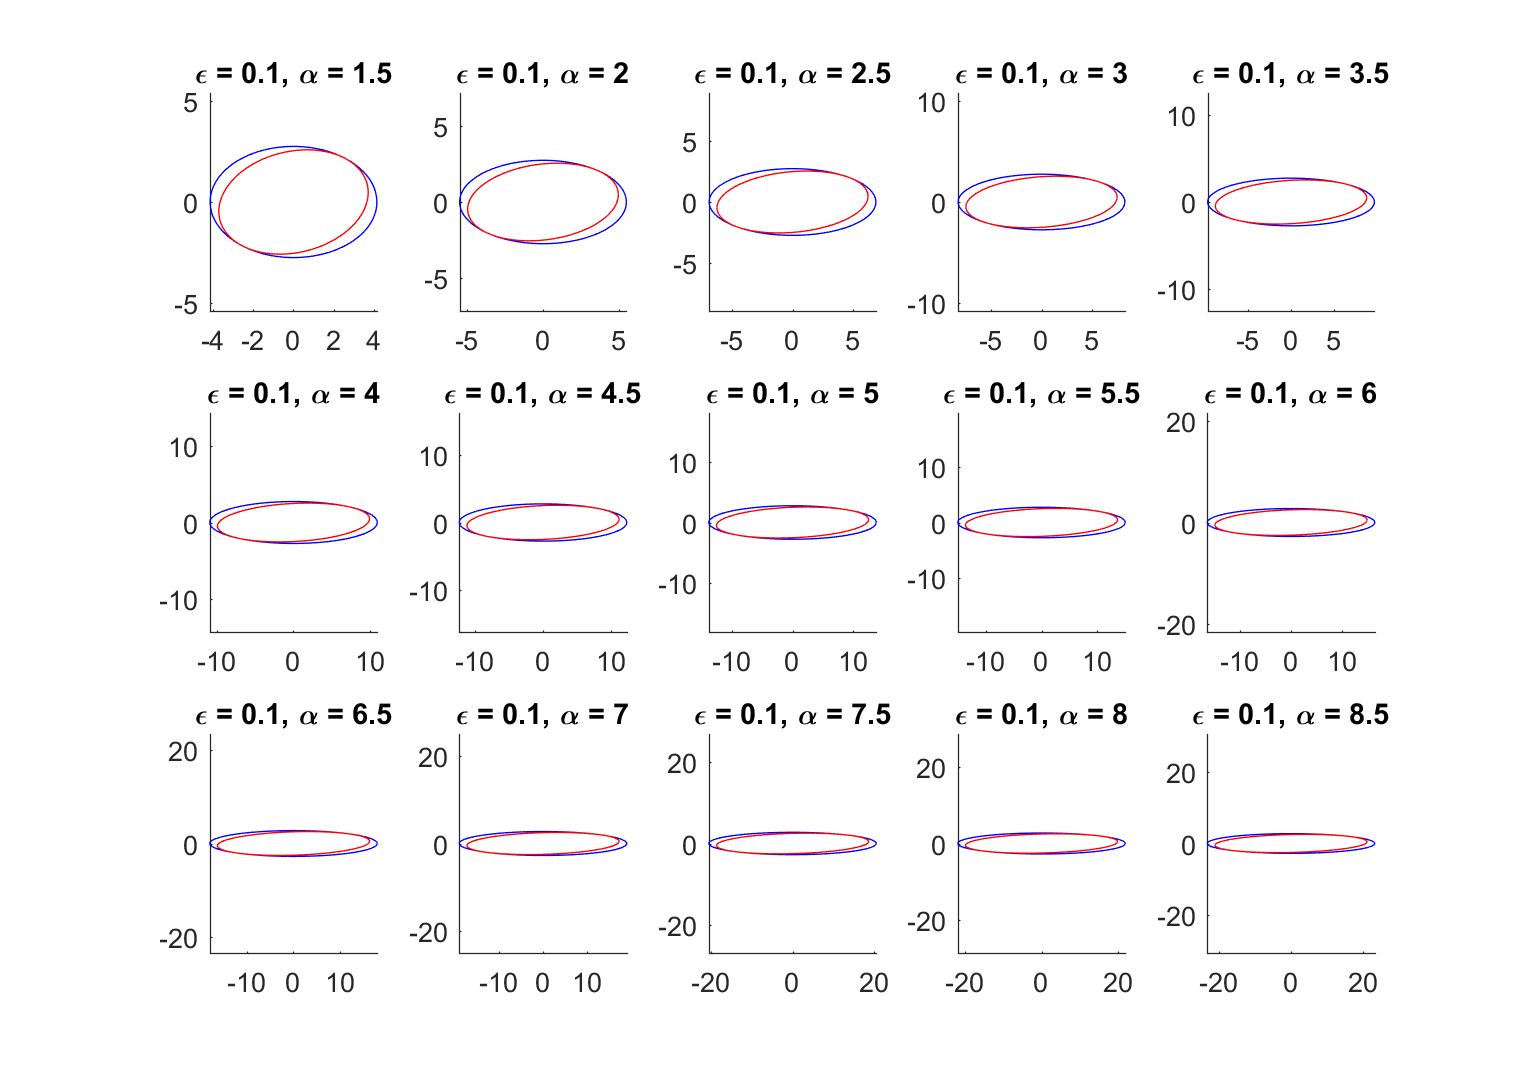
\includegraphics[scale = 0.17]{fig/closed-form_maxAngle-test_alpha.png}
\caption{Test with different values of aspect ratio $\alpha$, fixed $\epsilon = 0.1$}
\label{diff-alpha}
\end{figure}

\begin{figure}
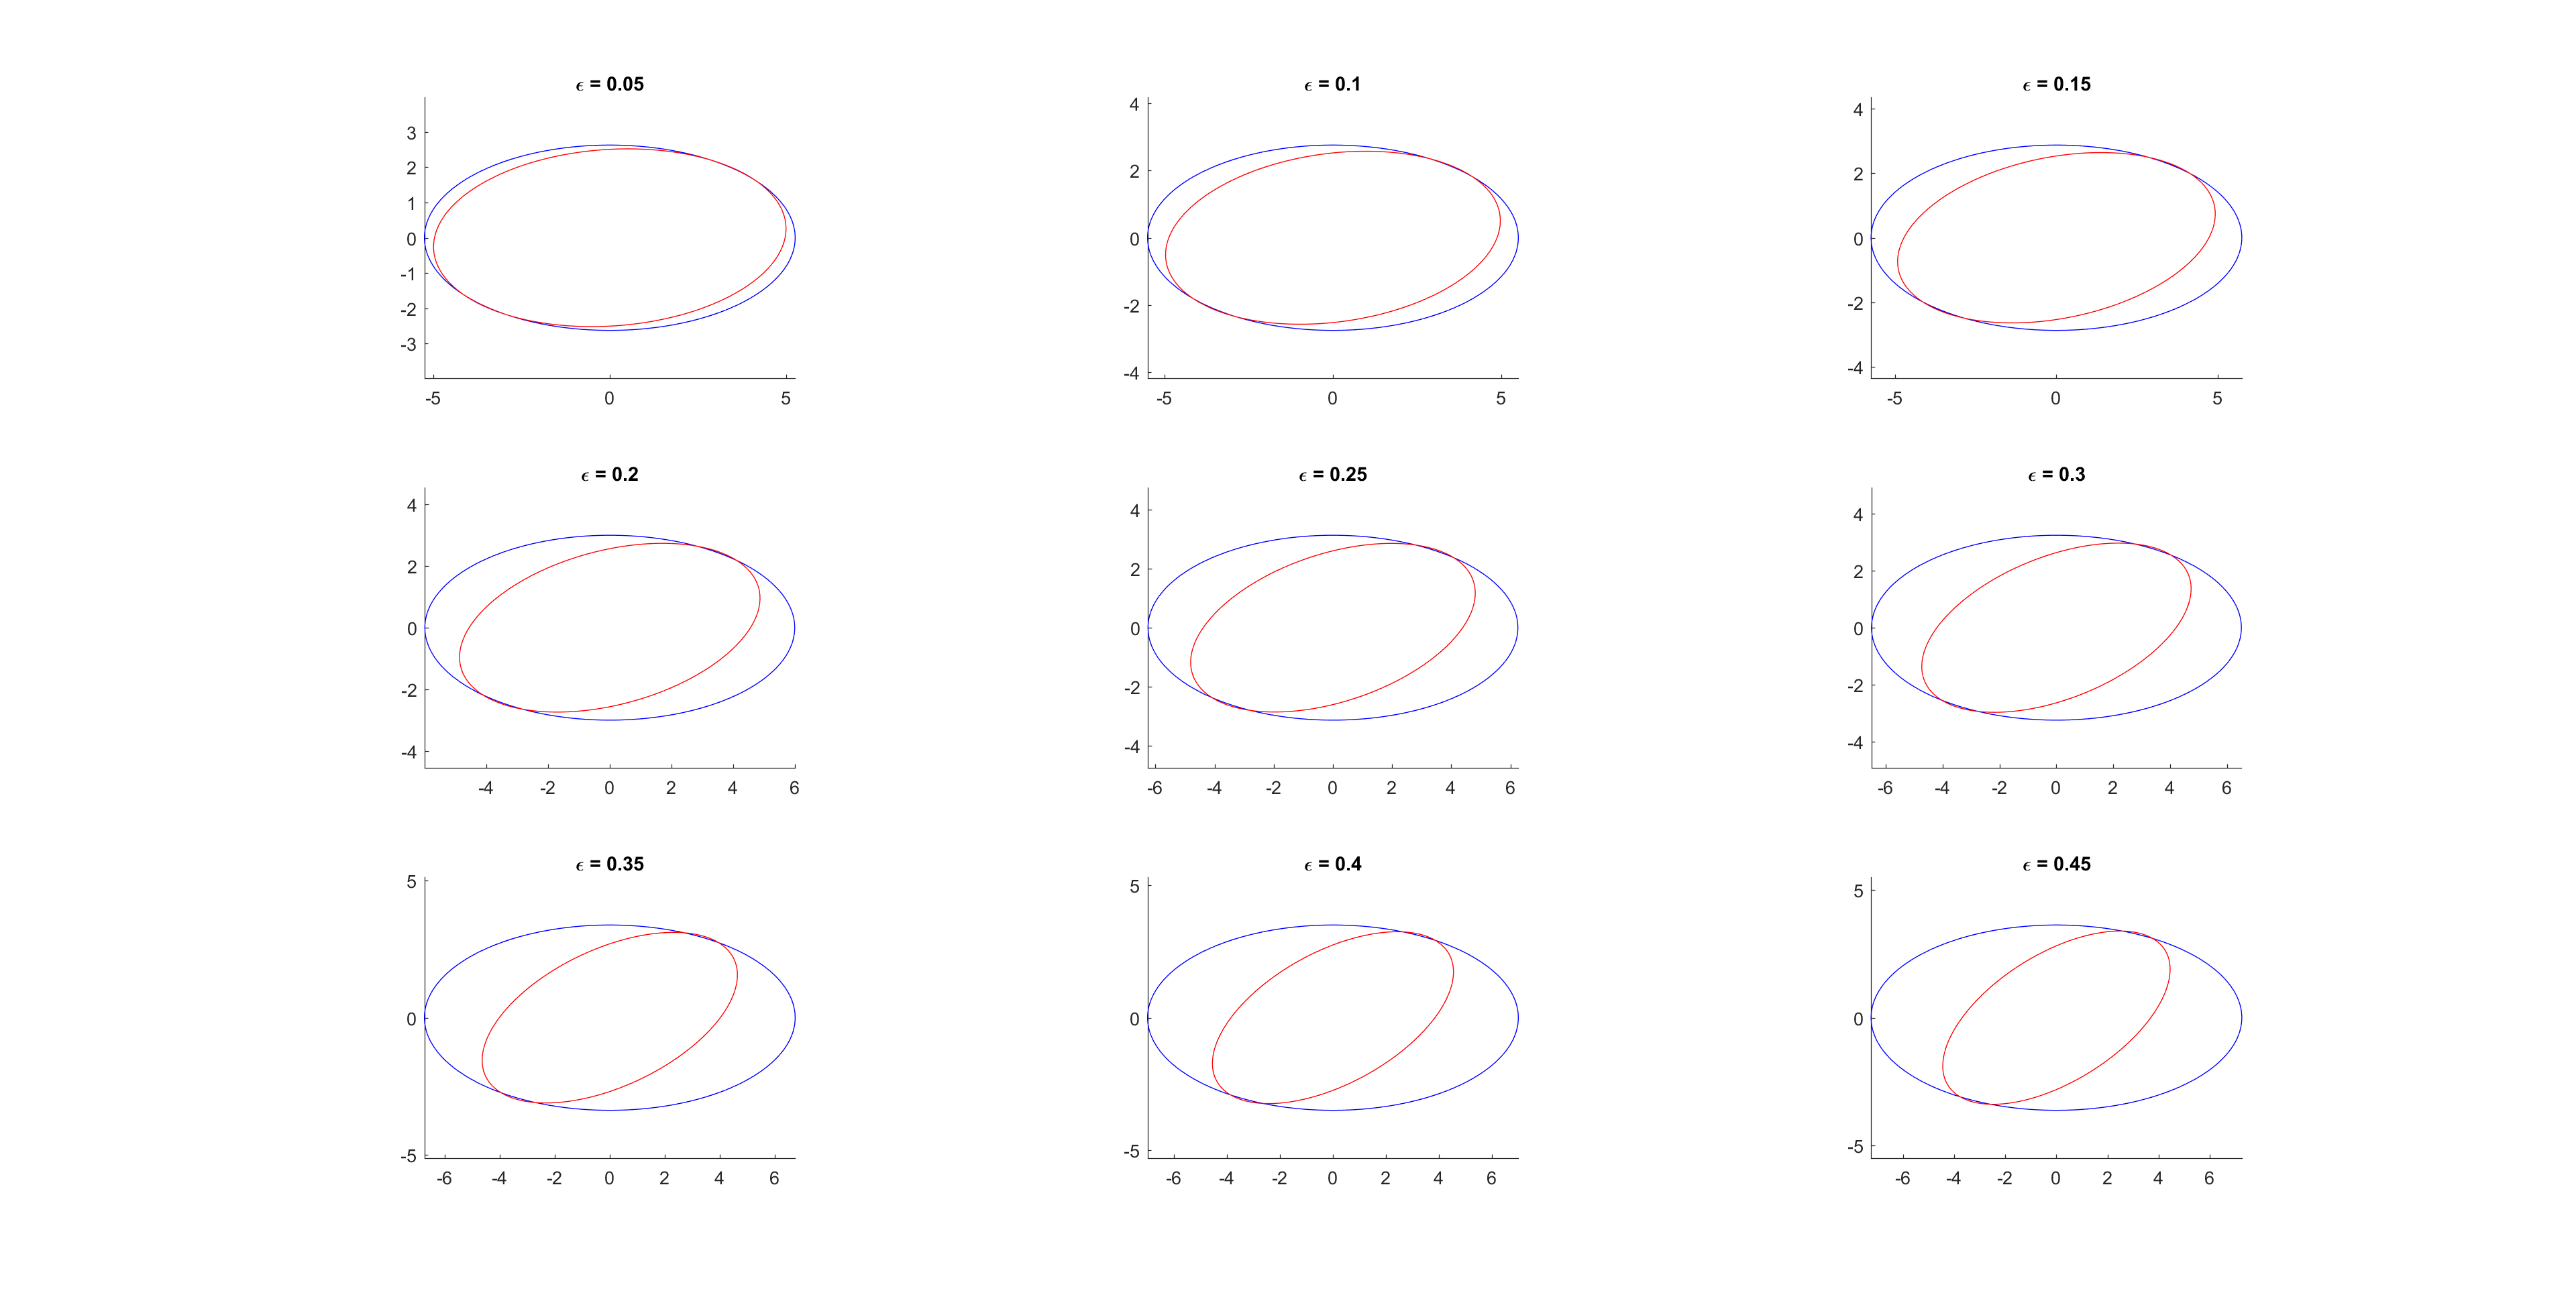
\includegraphics[scale = 0.17]{fig/closed-form_maxAngle-test_epsilon.png}
\caption{Test with different values of explode factor $\epsilon$, fixed $\alpha = 2$}
\label{diff-epi}
\end{figure}

\item {\bf Heuristic KC with twisted ellipsoid fit}\\
It is observed that the convex hull of the sample-based c-space of KC is twisted along x-axis. So we try to untwist the space along x-axis, fit a convex shape inside the sample-based convex hull, and twist back to get a better fit. 

At first, figure \ref{comp_cspace} is a comparison of twisted and untwisted C-Space.
\begin{figure}
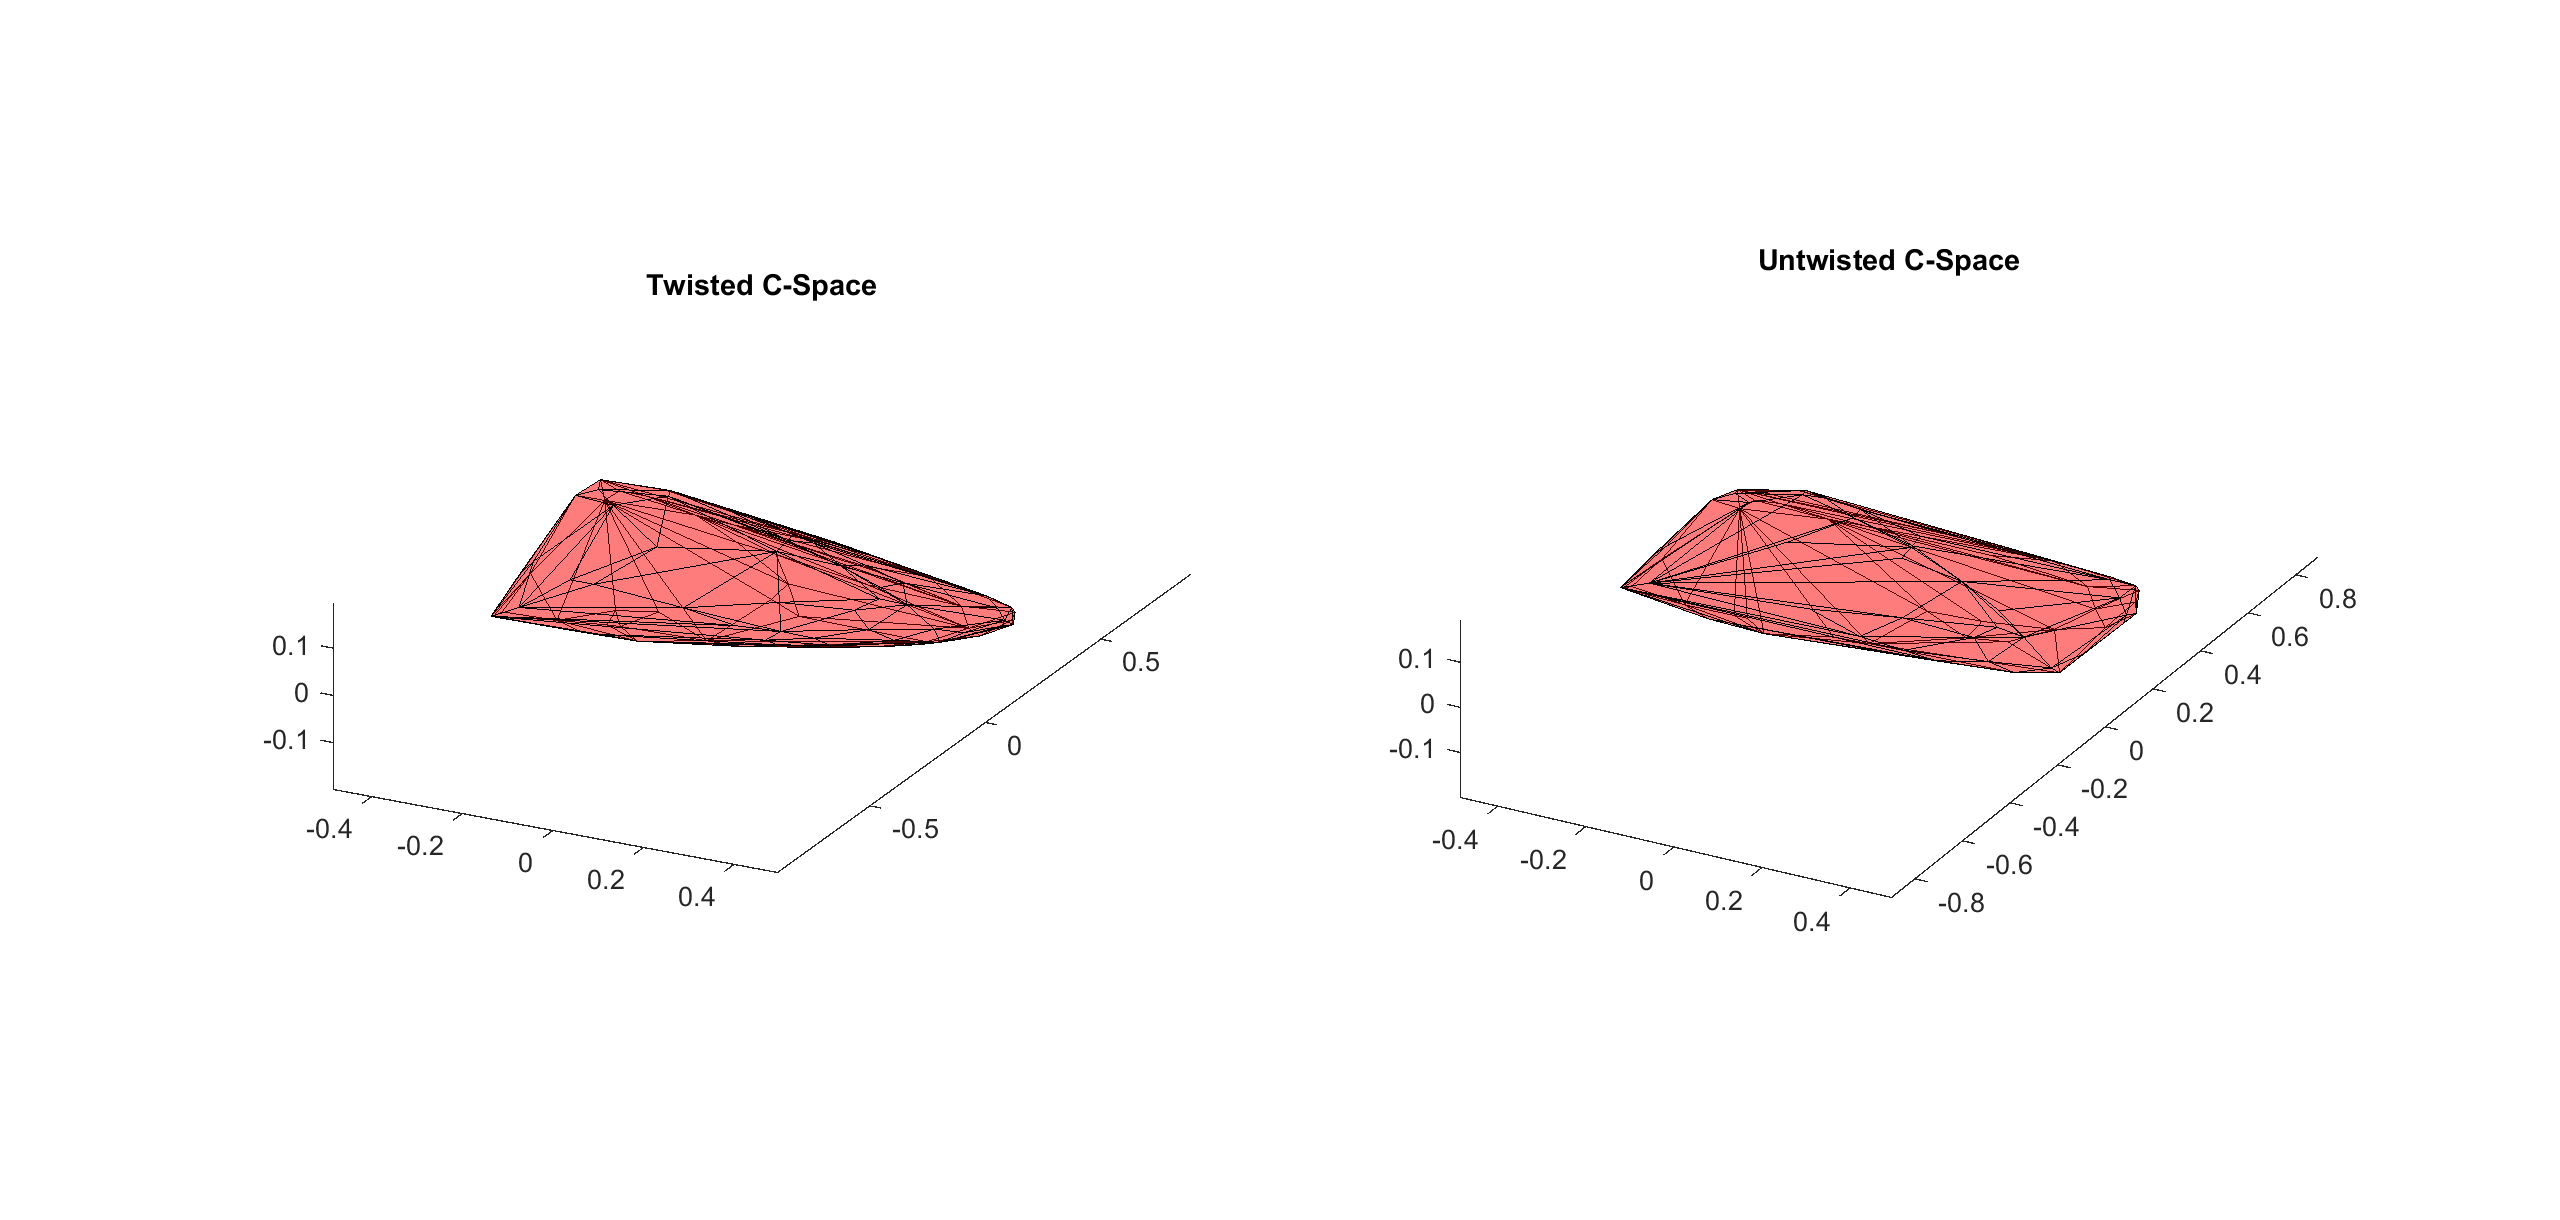
\includegraphics[scale=0.25]{fig/comparison_twist-untwist_c-space.png}
\caption{Comparison of twisted and untwisted c-space}
\label{comp_cspace}
\end{figure}
Note that the untwisting angle $\beta$ is set manually, which is proportional to the x-coordinate, i.e $\beta = kx$, where $k$ is set by observation, so the next step is to find an automatic way to set the angle. Also, $\beta$ might also be proportional to a higher order of $x$ so that the untwisted version of the c-space might look better.

For the current experiment, I fit an ellipsoid into the untwisted c-space, with the equation $\frac{x^2}{(a_1 \epsilon)^2} + \frac{y^2}{(a_2 \epsilon)^2} + \frac{\theta^2}{\phi^2} = 1$, where each denominator ($a_1 \epsilon, a_2 \epsilon, \phi$) is the maximum displacement in the corresponding axis in c-space.

Figure \ref{twist_fit} is one example of the heuristic fit.
\begin{figure}
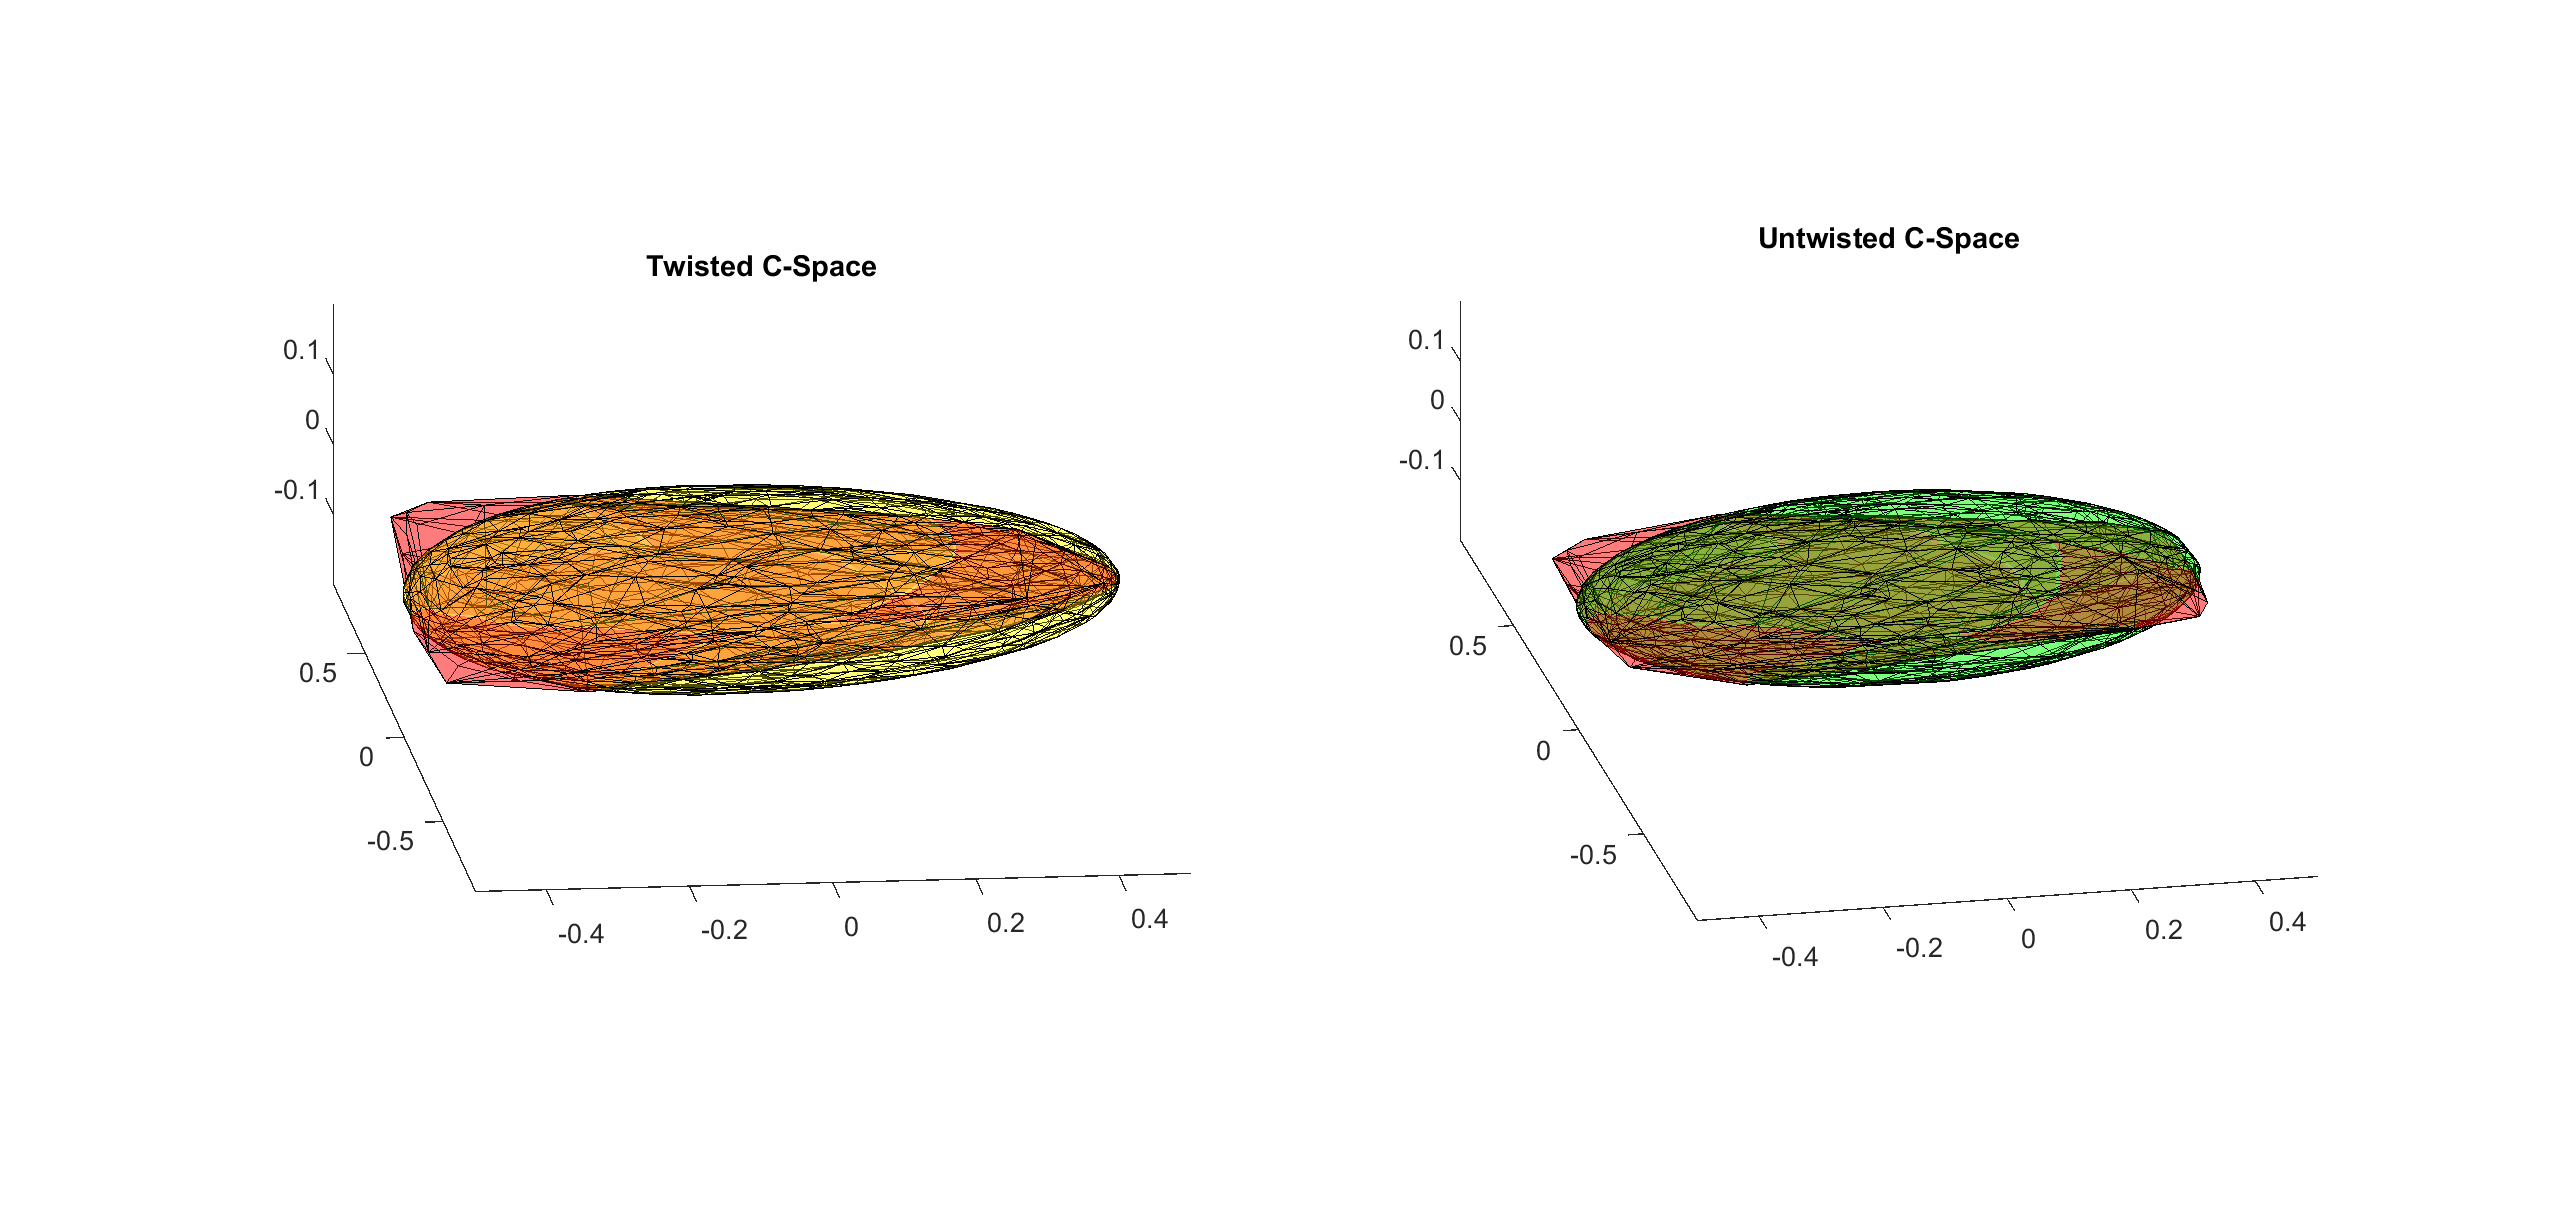
\includegraphics[scale = 0.25]{fig/twist-untwist_c-space_fit.png}
\caption{heuristic fit, with parameters: $a_2 = 2.5$, $\alpha = 2$, $\epsilon = 0.1$, $\beta = 0.6x$}
\label{twist_fit}
\end{figure}
The fitted ellipsoid exceeds the range of the convex hull, which is infeasible. To solve this, we could define a scale factor to the ellipsoid parameters, factor can be different for each parameter, but this still needs manually observation. Figure \ref{fit_scaled} shows the scaled heuristic fit, with $\theta$ scaled only.

\begin{figure}
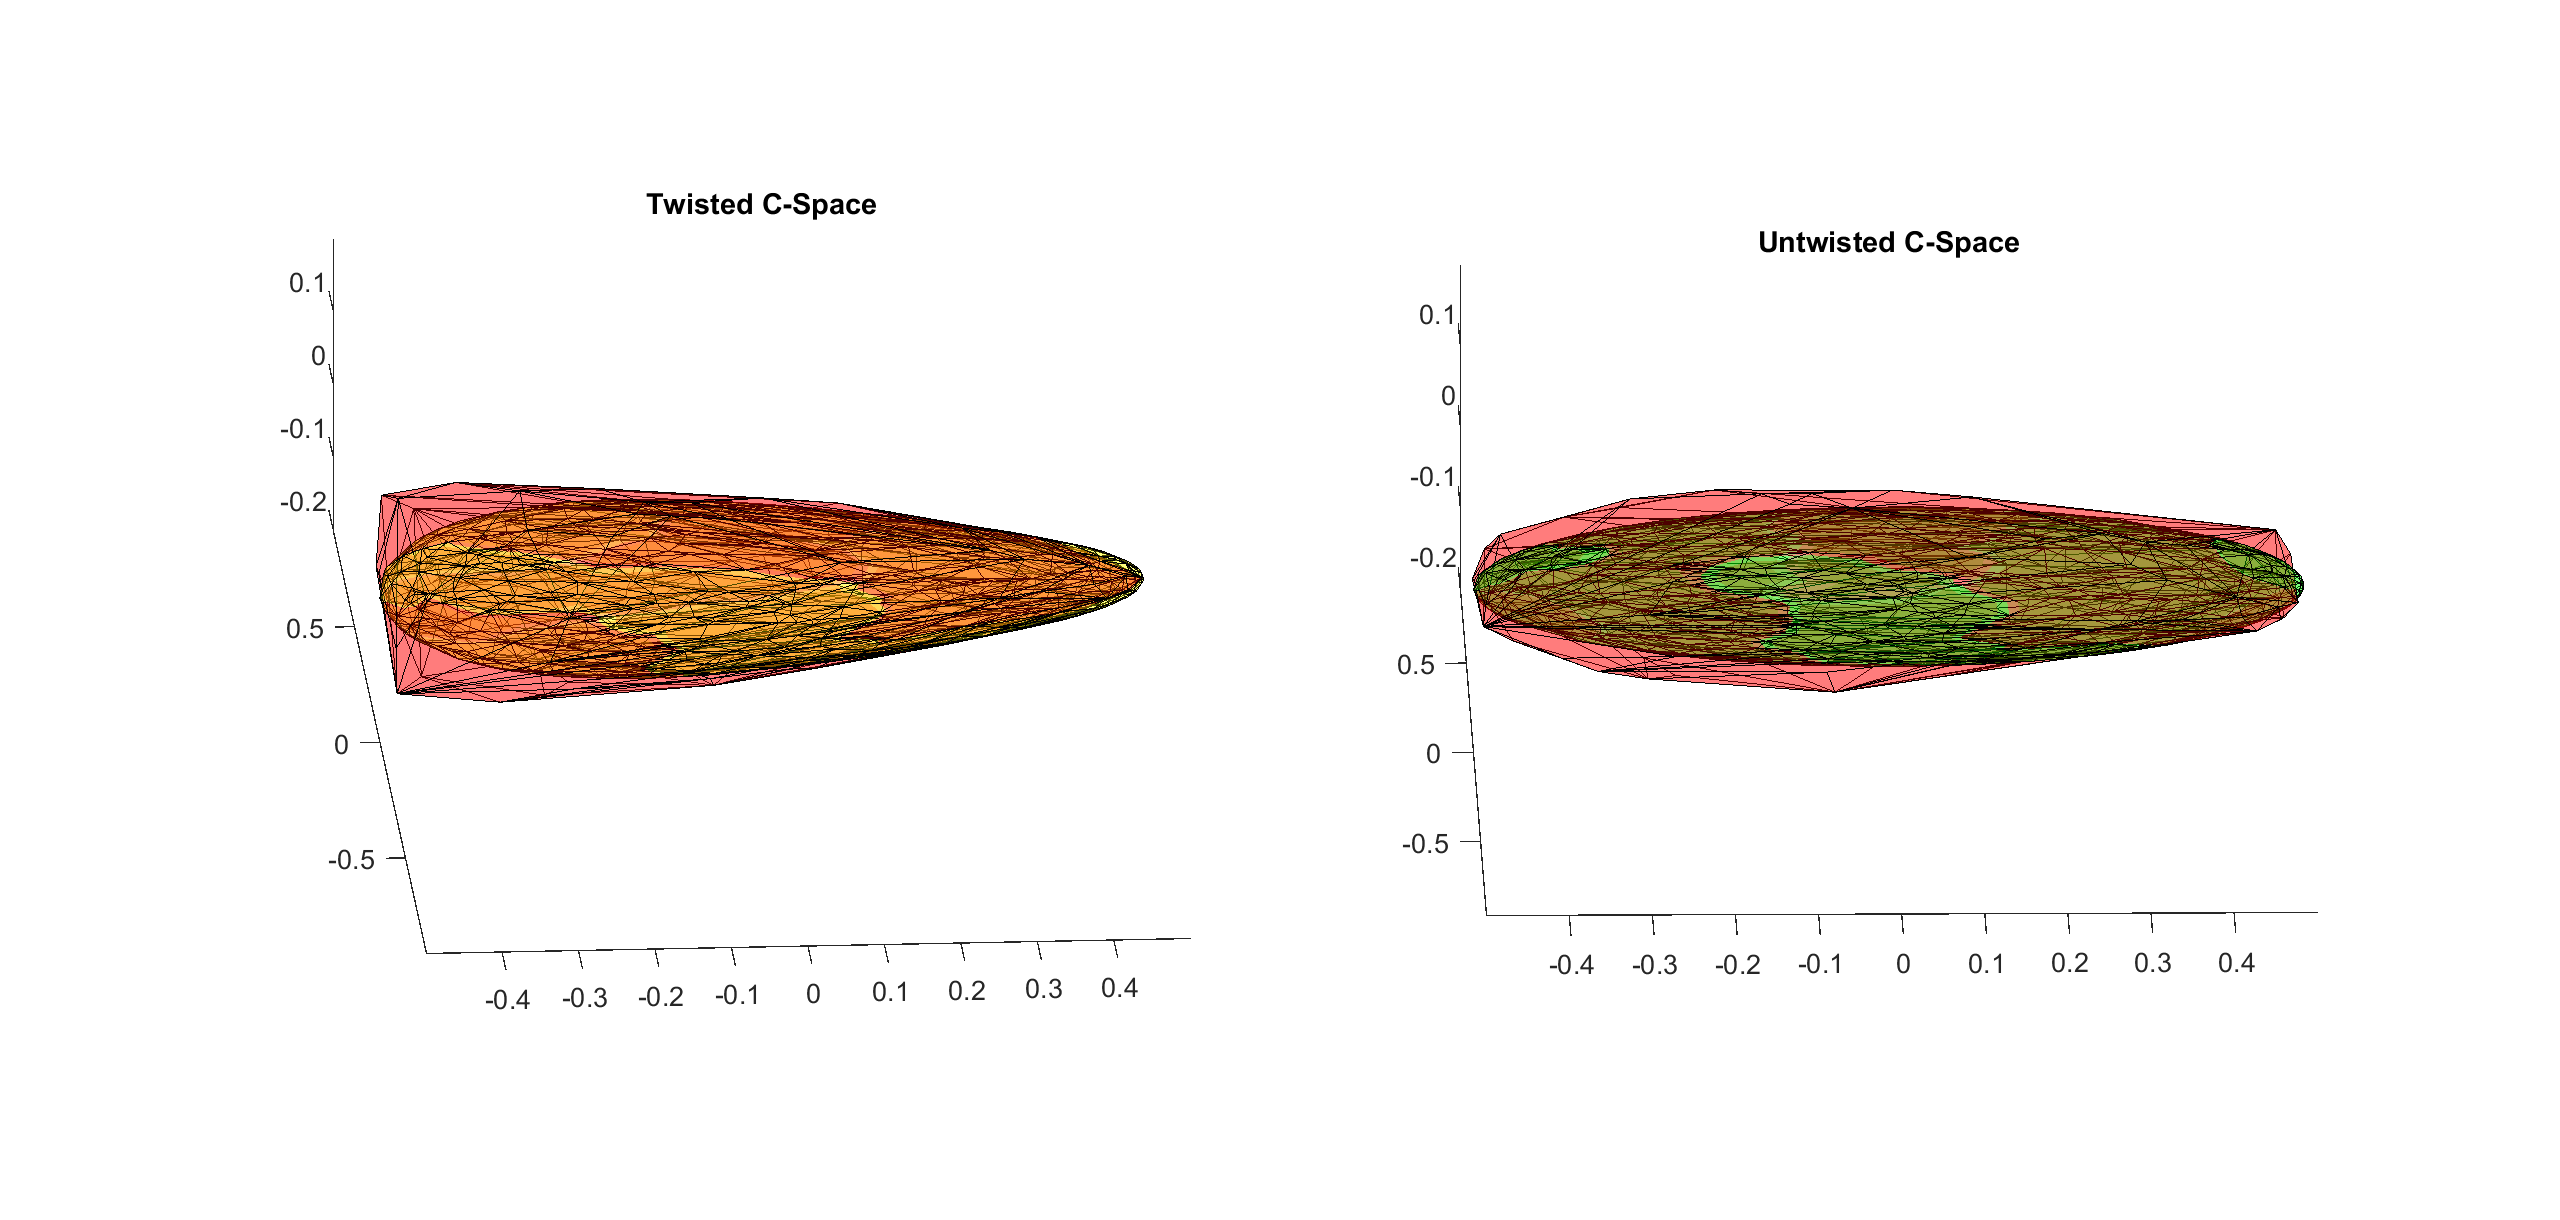
\includegraphics[scale = 0.25]{fig/twist-untwist_c-space_fit_scaled.png}
\caption{heuristic fit, with parameters: $a_2 = 2.5$, $\alpha = 2$, $\epsilon = 0.1$, $\beta = 0.6x$, scale factor: 0.6}
\label{fit_scaled}
\end{figure}

\item {\bf Heuristic fit with different aspect ratios}
Each time we change the aspect ratio $\alpha$, we need to manually change the factor $k$ of twisting function $\beta = kx$ correspondingly. Table \ref{table_diff_ratio} lists the aspect ratios and the corresponding twisting factors.

\begin{center}
\begin{tabular}{ c|c|c|c|c|c|c } 
 \hline
 Aspect ratio $\alpha$ & 1.5  & 1.8 & 2   & 2.2 & 2.5  & 3    \\
 \hline
 Twisting factor $k$   & 1.75 & 1   & 0.6 & 0.5 & 0.35 & 0.25 \\
 \hline
\end{tabular}
\label{table_diff_ratio}
\end{center}

Figures \ref{fit_scaled1.5}, \ref{fit_scaled1.8}, \ref{fit_scaled2.2}, \ref{fit_scaled2.5} and \ref{fit_scaled3} show the heuristic fit with different aspect ratios.

\begin{figure}
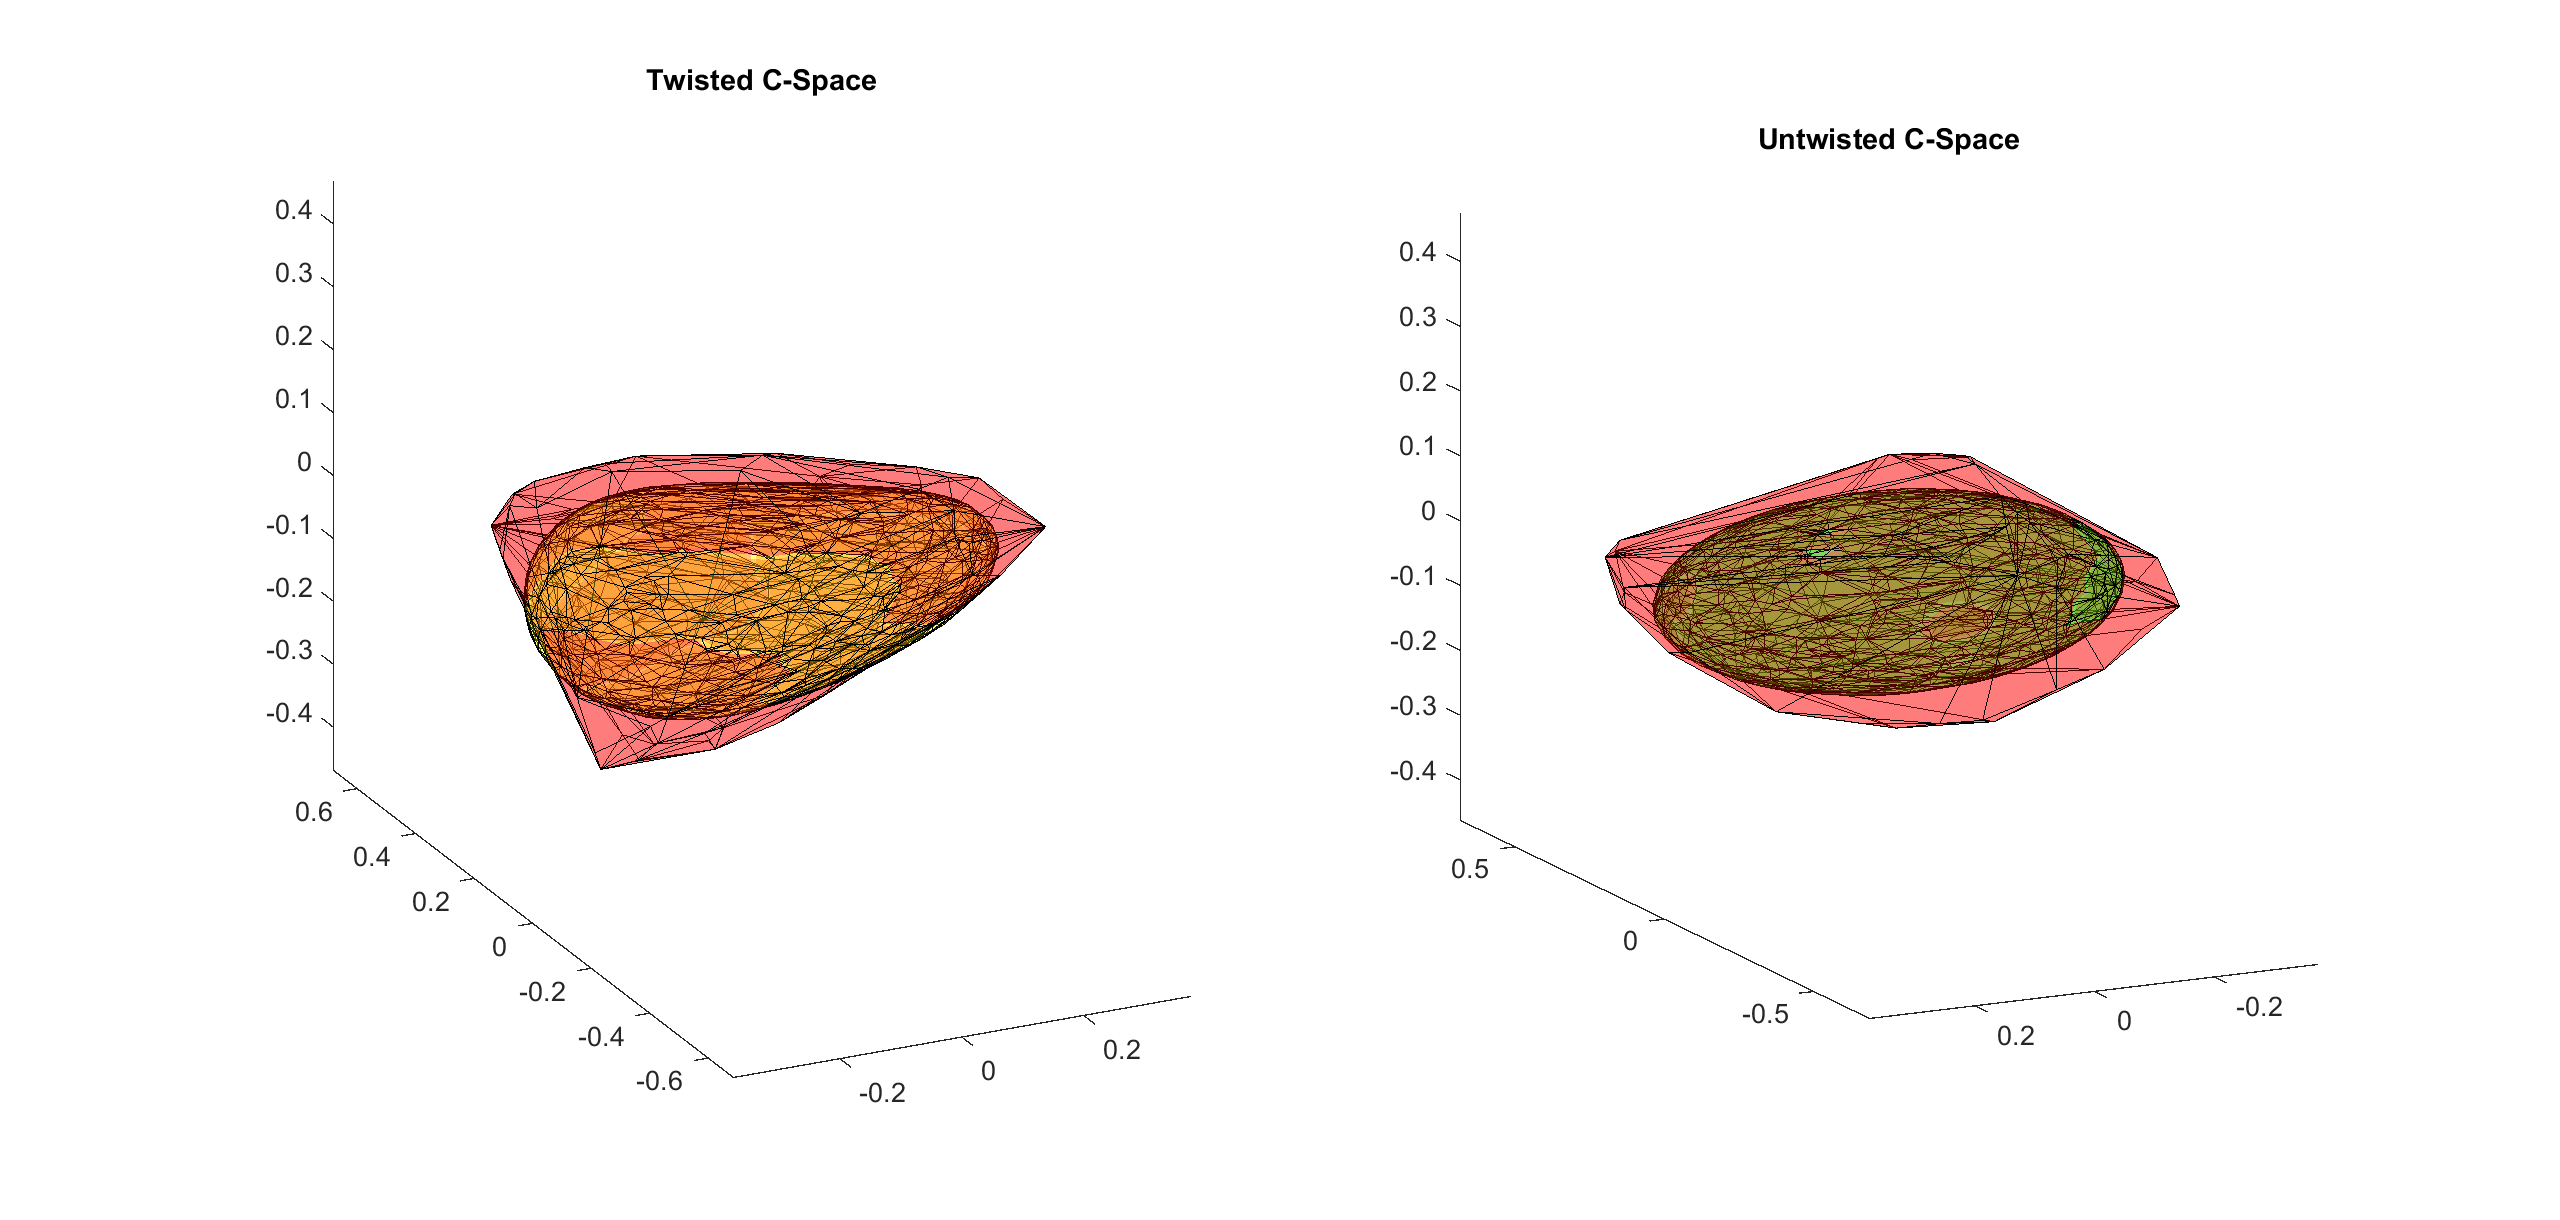
\includegraphics[scale = 0.25]{fig/twist-untwist_c-space_fit_scaled_ratio1_5.png}
\caption{heuristic fit, with parameters: $a_2 = 2.5$, $\alpha = 1.5$, $\epsilon = 0.1$, $\beta = 0.75x$, scale factor: 0.6}
\label{fit_scaled1.5}
\end{figure}
\begin{figure}
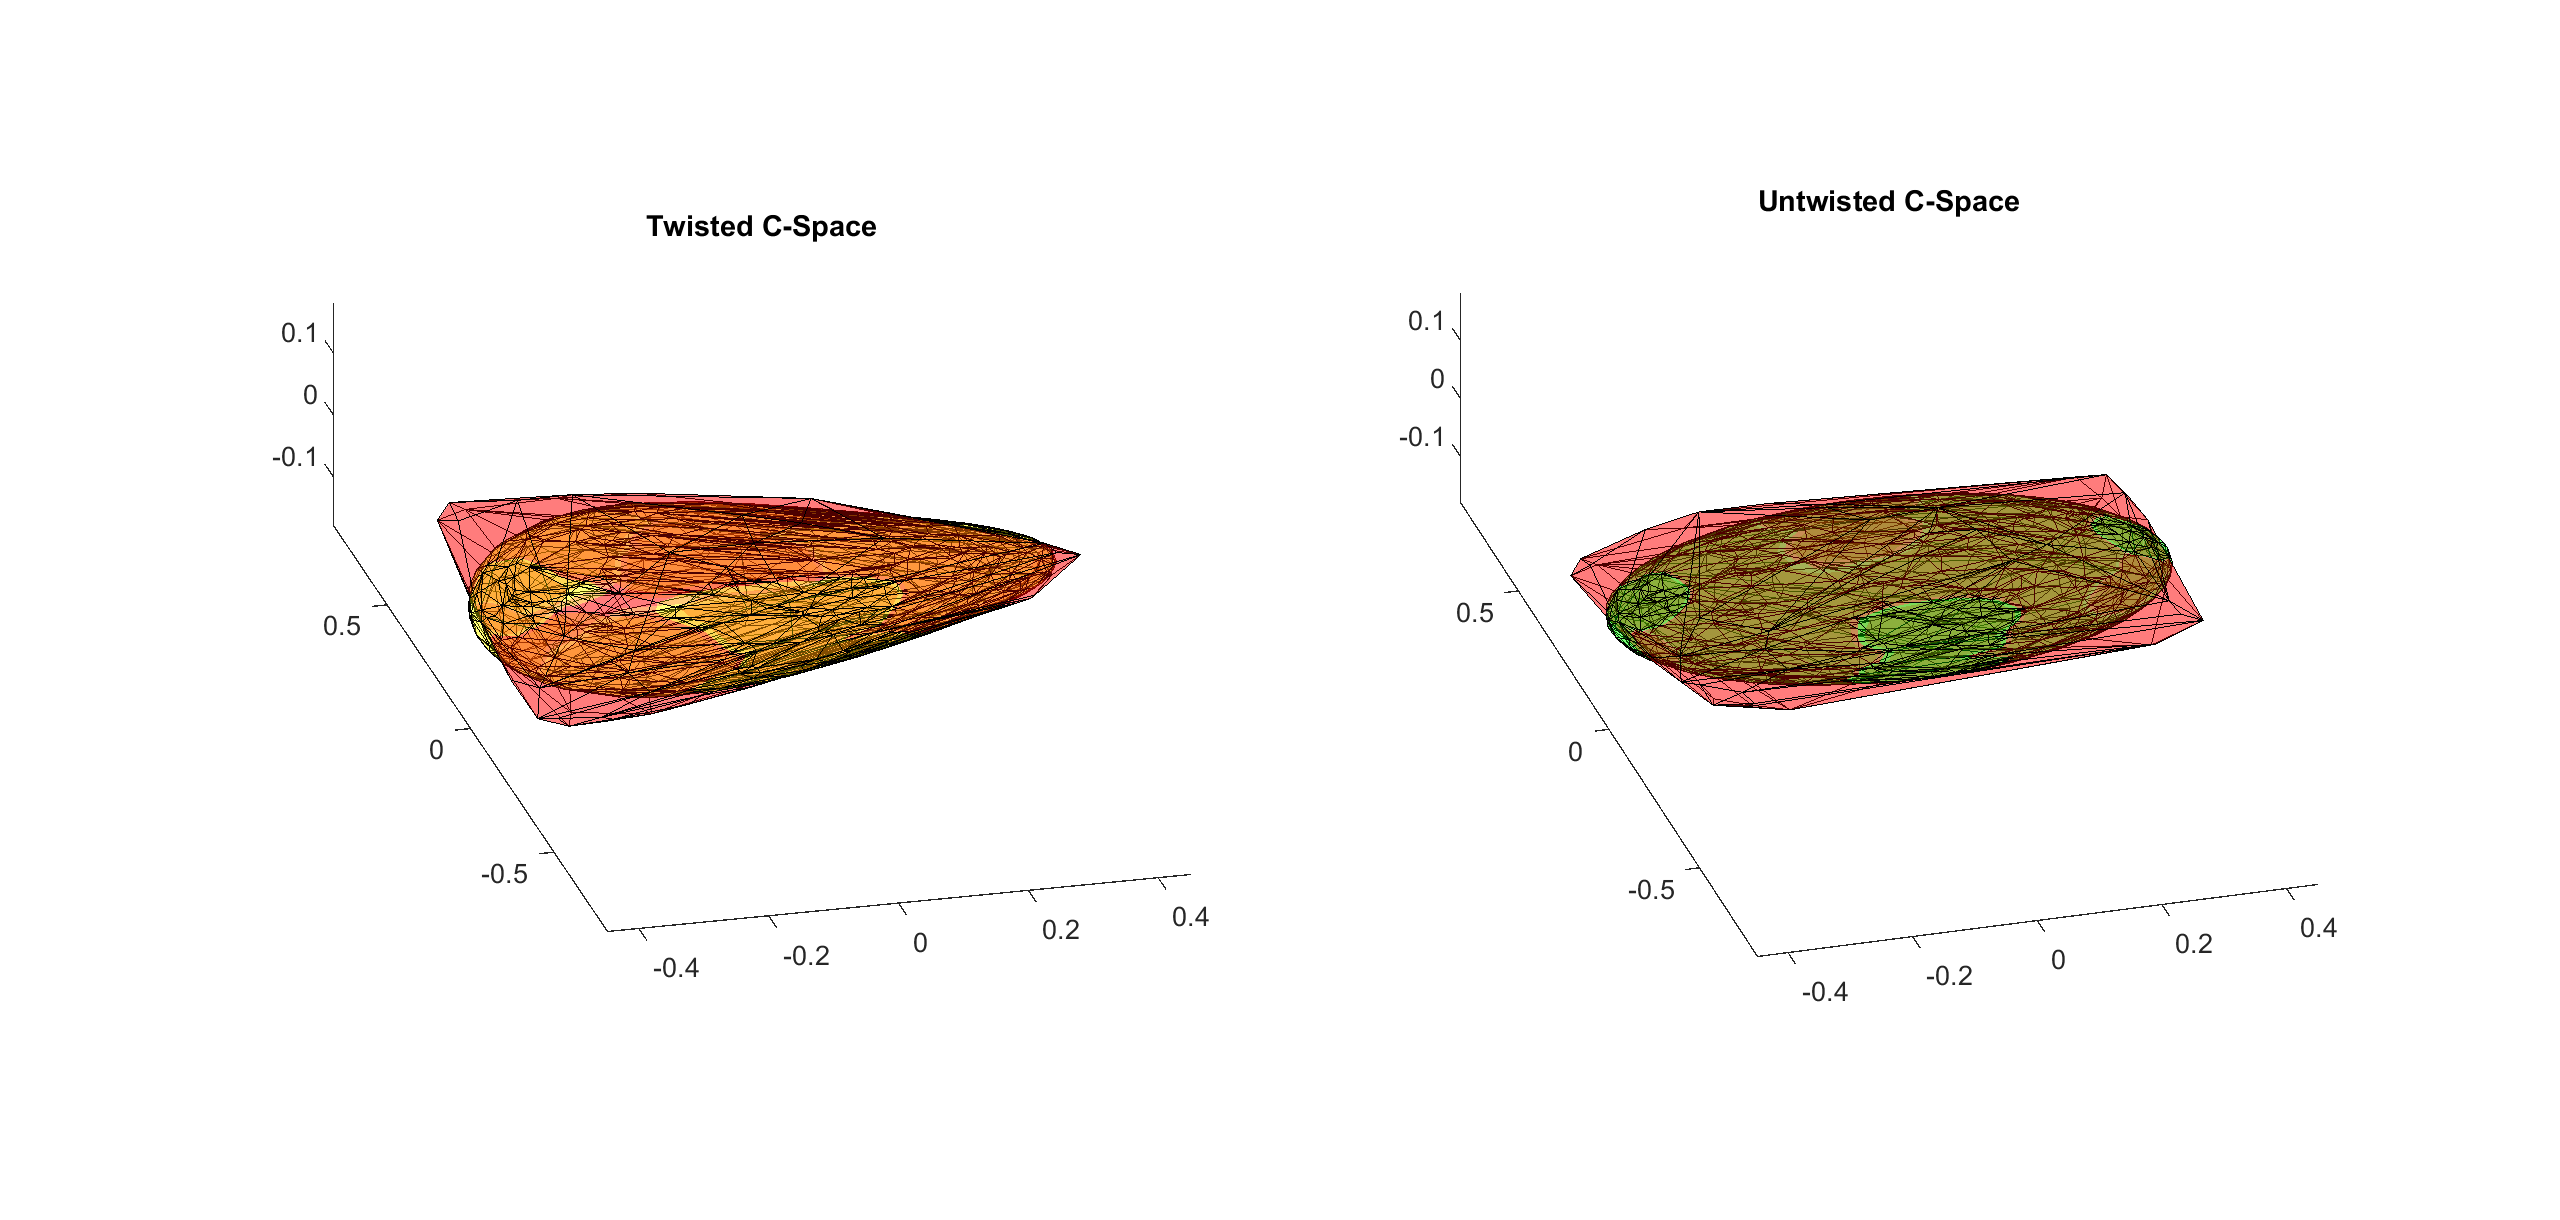
\includegraphics[scale = 0.25]{fig/twist-untwist_c-space_fit_scaled_ratio1_8.png}
\caption{heuristic fit, with parameters: $a_2 = 2.5$, $\alpha = 1.8$, $\epsilon = 0.1$, $\beta = x$, scale factor: 0.6}
\label{fit_scaled1.8}
\end{figure}
\begin{figure}
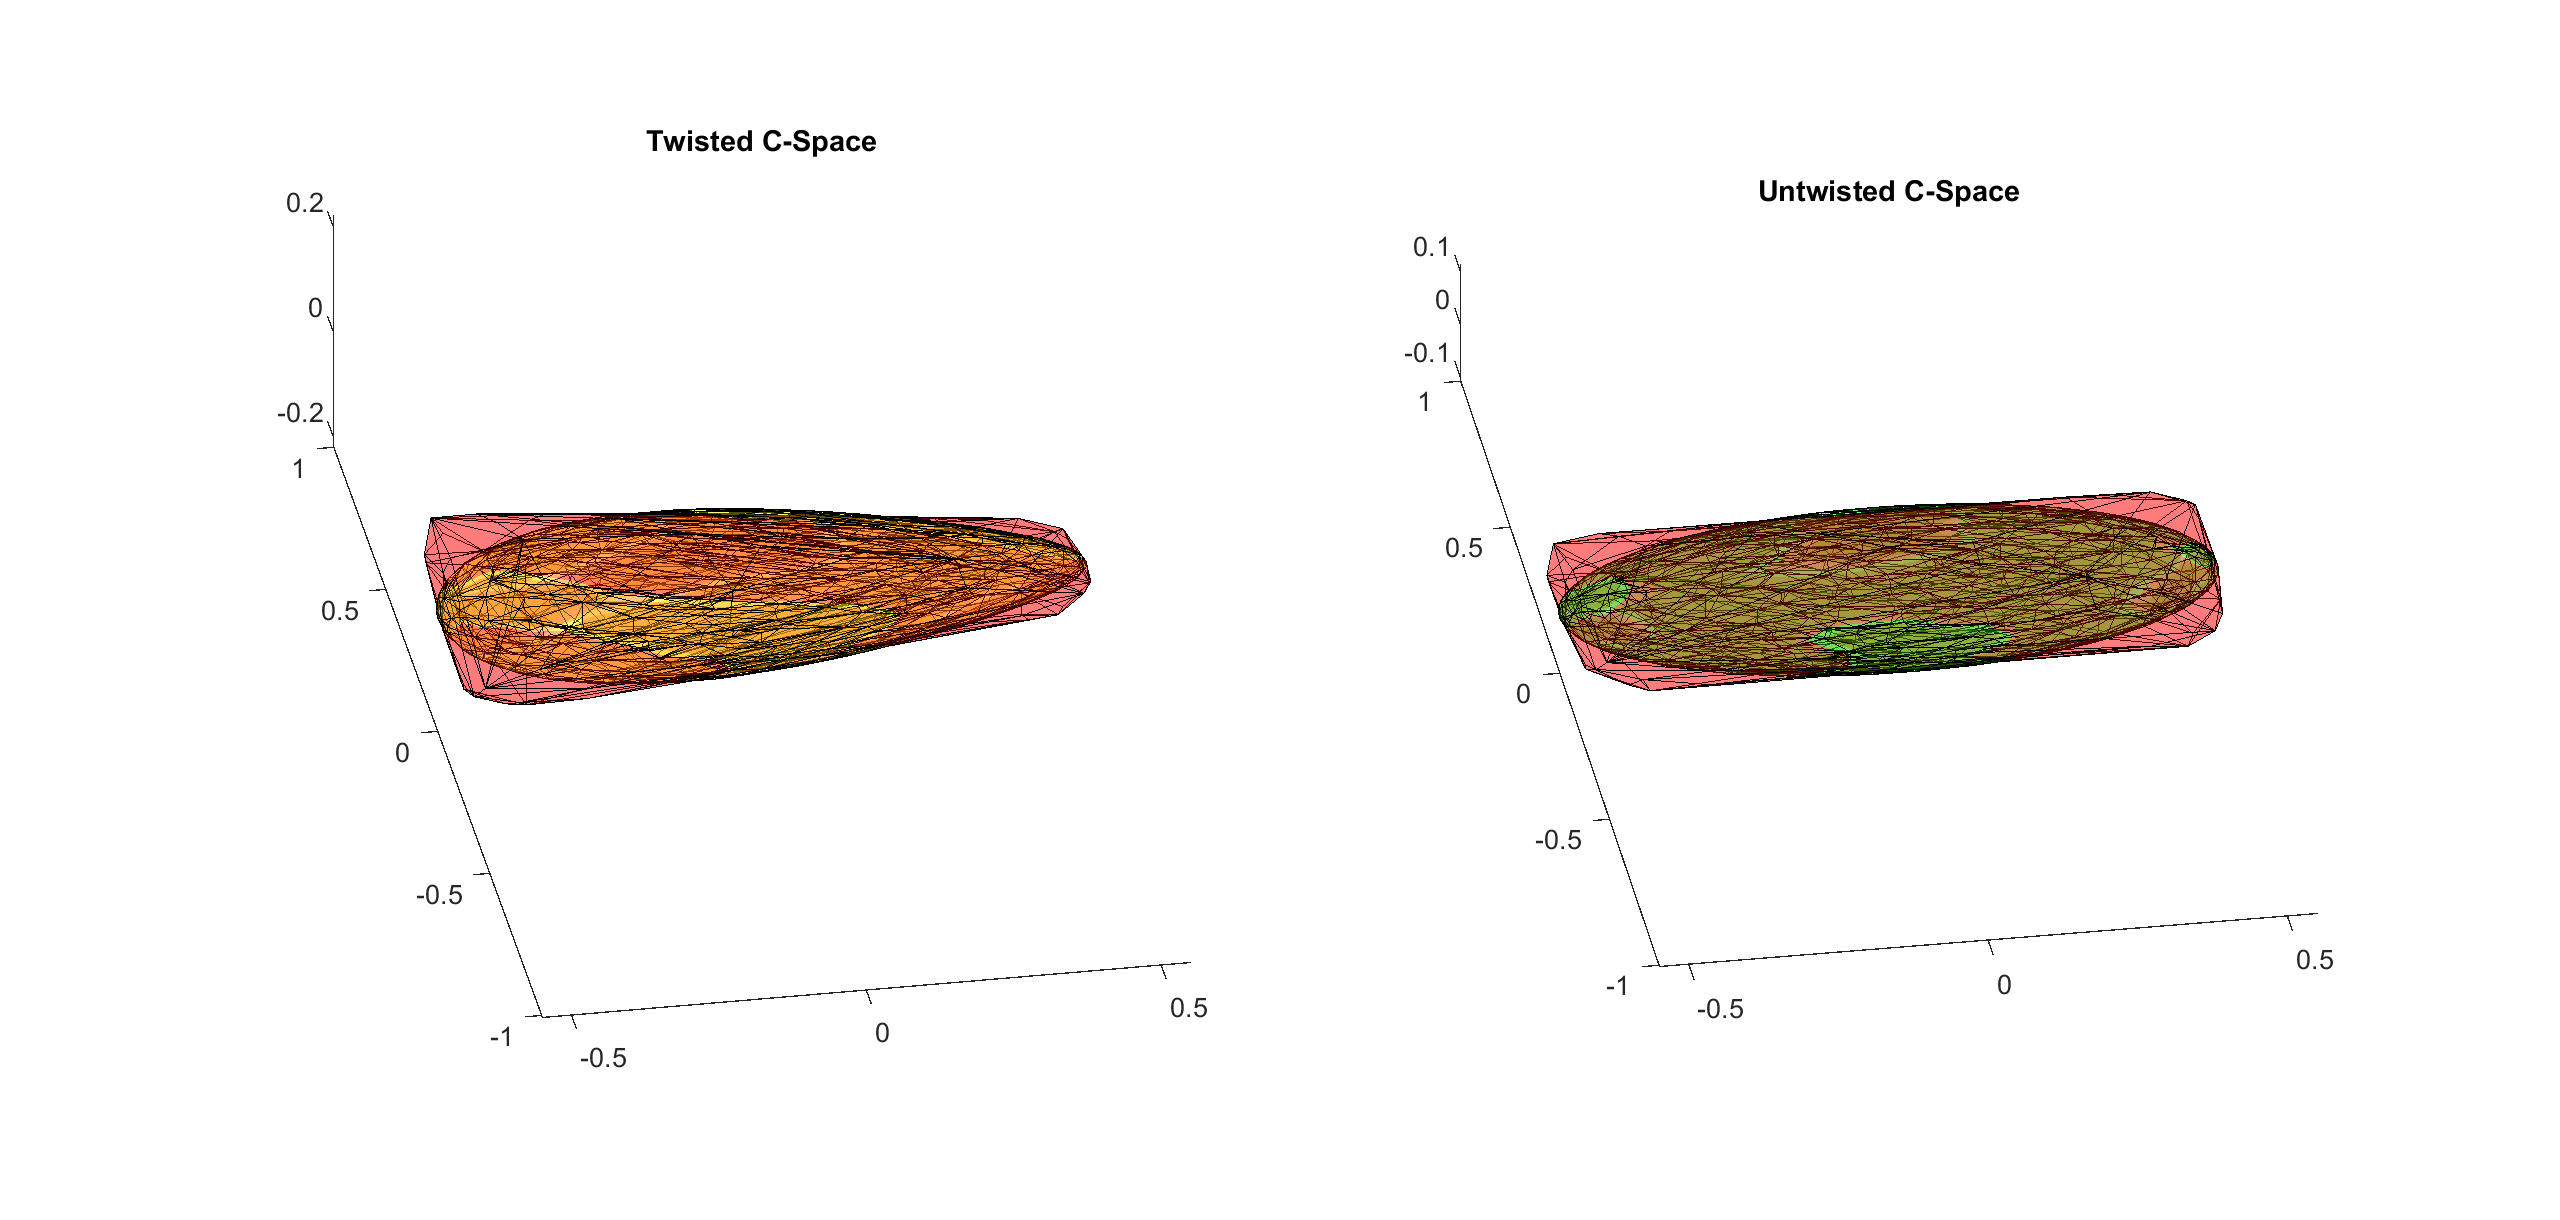
\includegraphics[scale = 0.25]{fig/twist-untwist_c-space_fit_scaled_ratio2_2.png}
\caption{heuristic fit, with parameters: $a_2 = 1.5$, $\alpha = 2.2$, $\epsilon = 0.1$, $\beta = 0.5x$, scale factor: 0.6}
\label{fit_scaled2.2}
\end{figure}
\begin{figure}
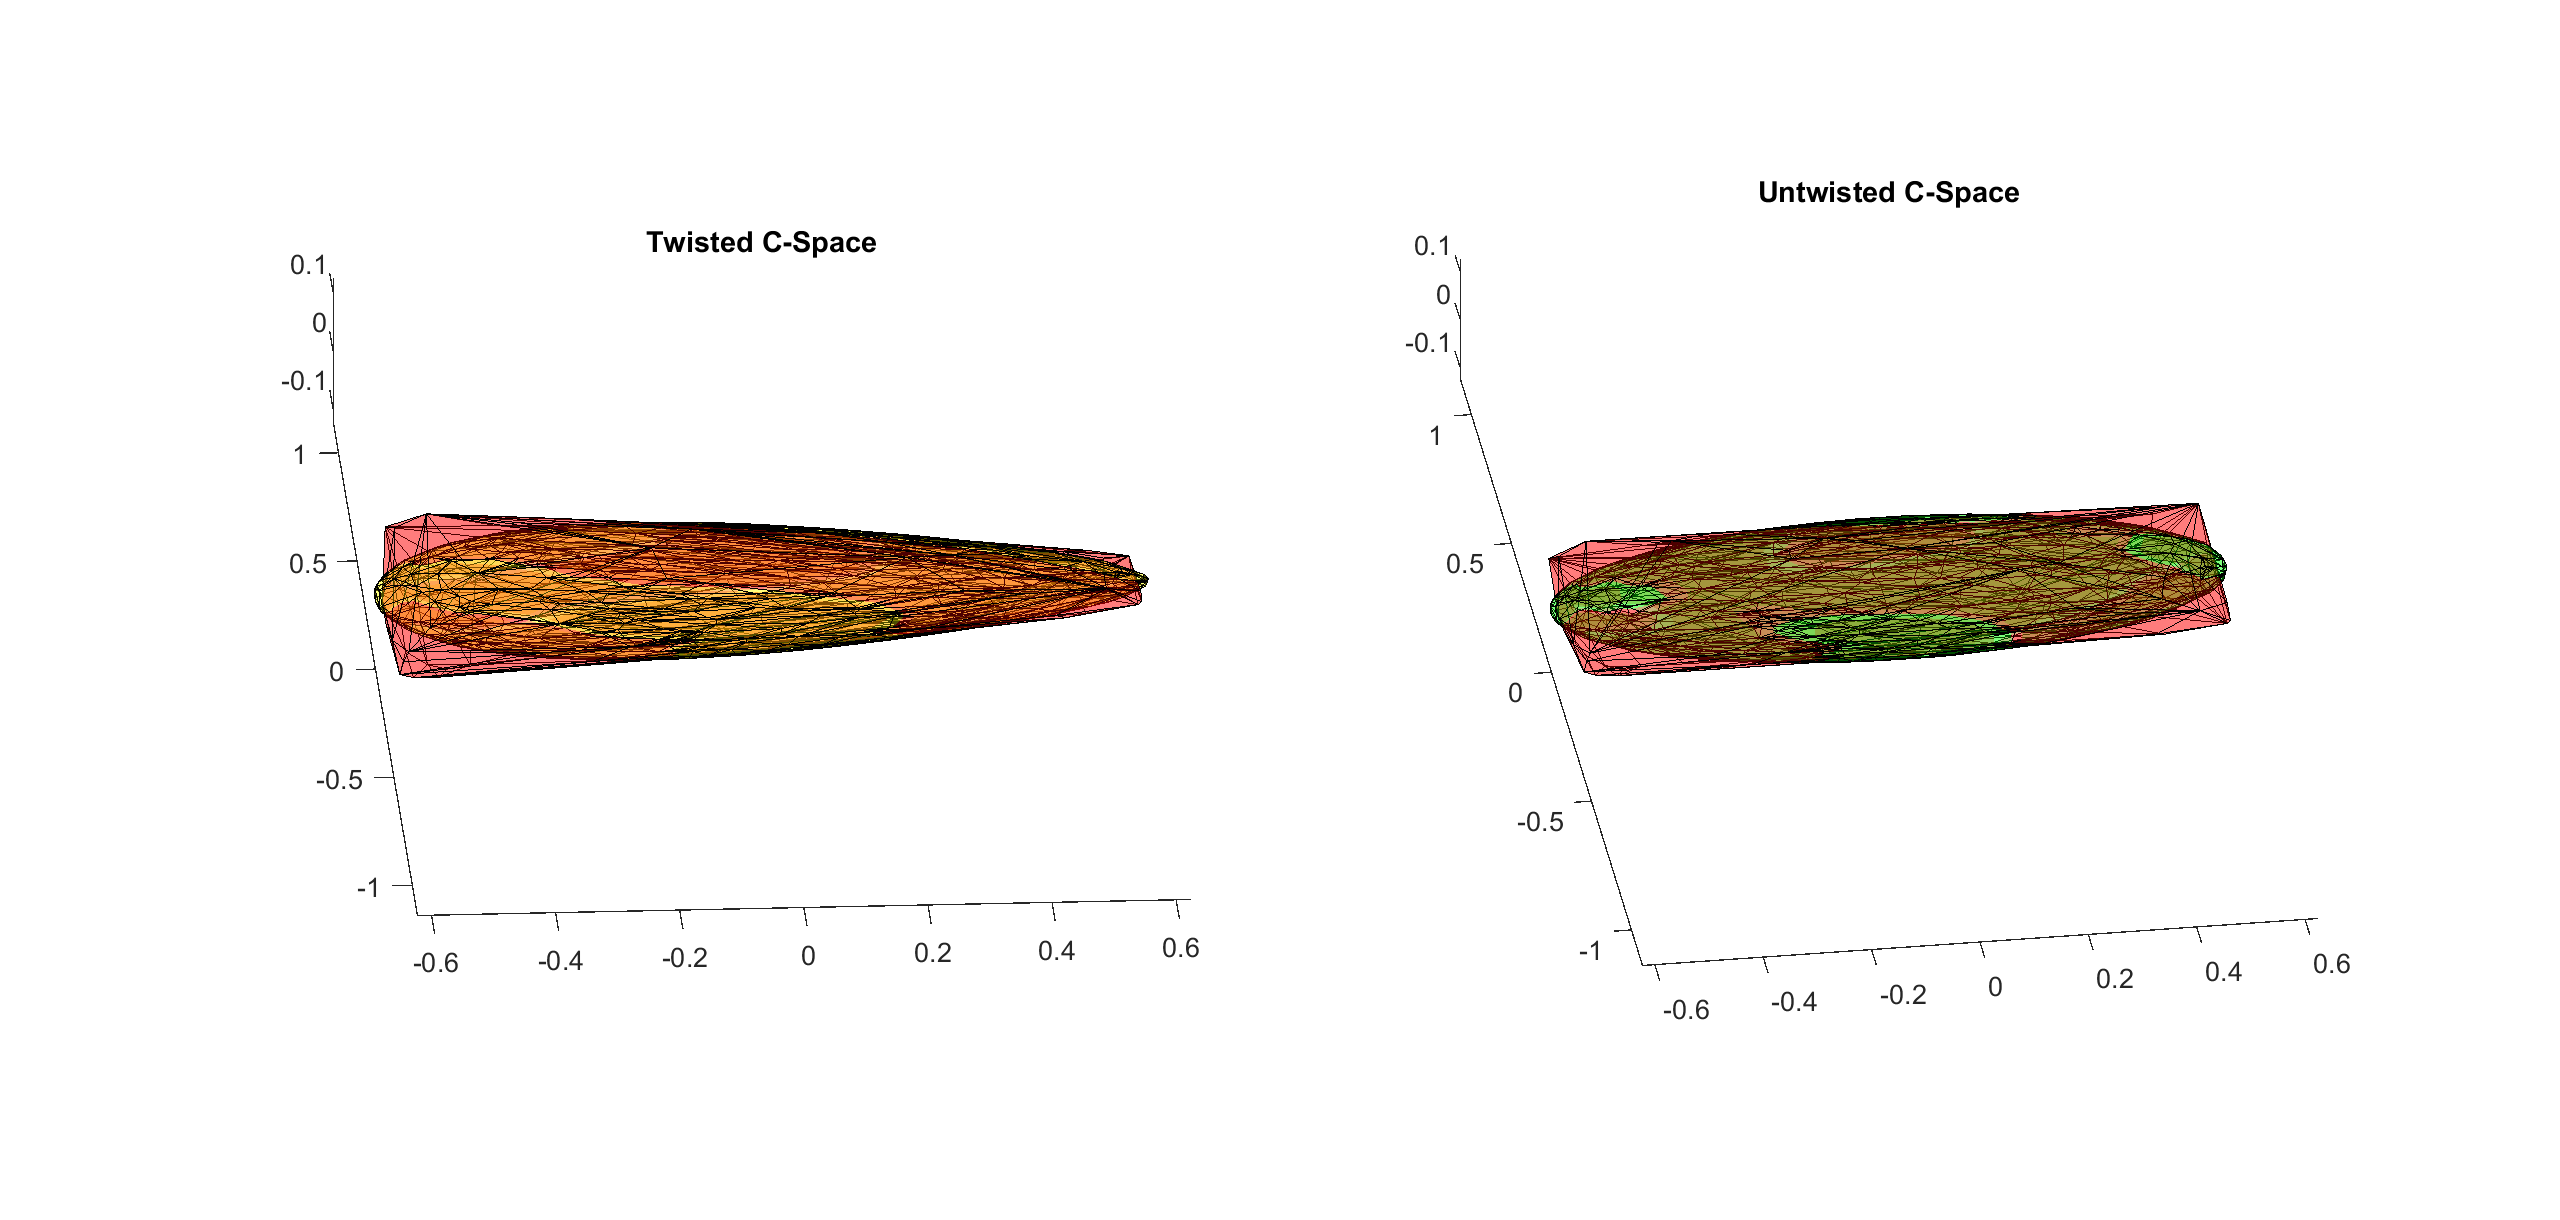
\includegraphics[scale = 0.25]{fig/twist-untwist_c-space_fit_scaled_ratio2_5.png}
\caption{heuristic fit, with parameters: $a_2 = 1.5$, $\alpha = 2.5$, $\epsilon = 0.1$, $\beta = 0.35x$, scale factor: 0.6}
\label{fit_scaled2.5}
\end{figure}
\begin{figure}
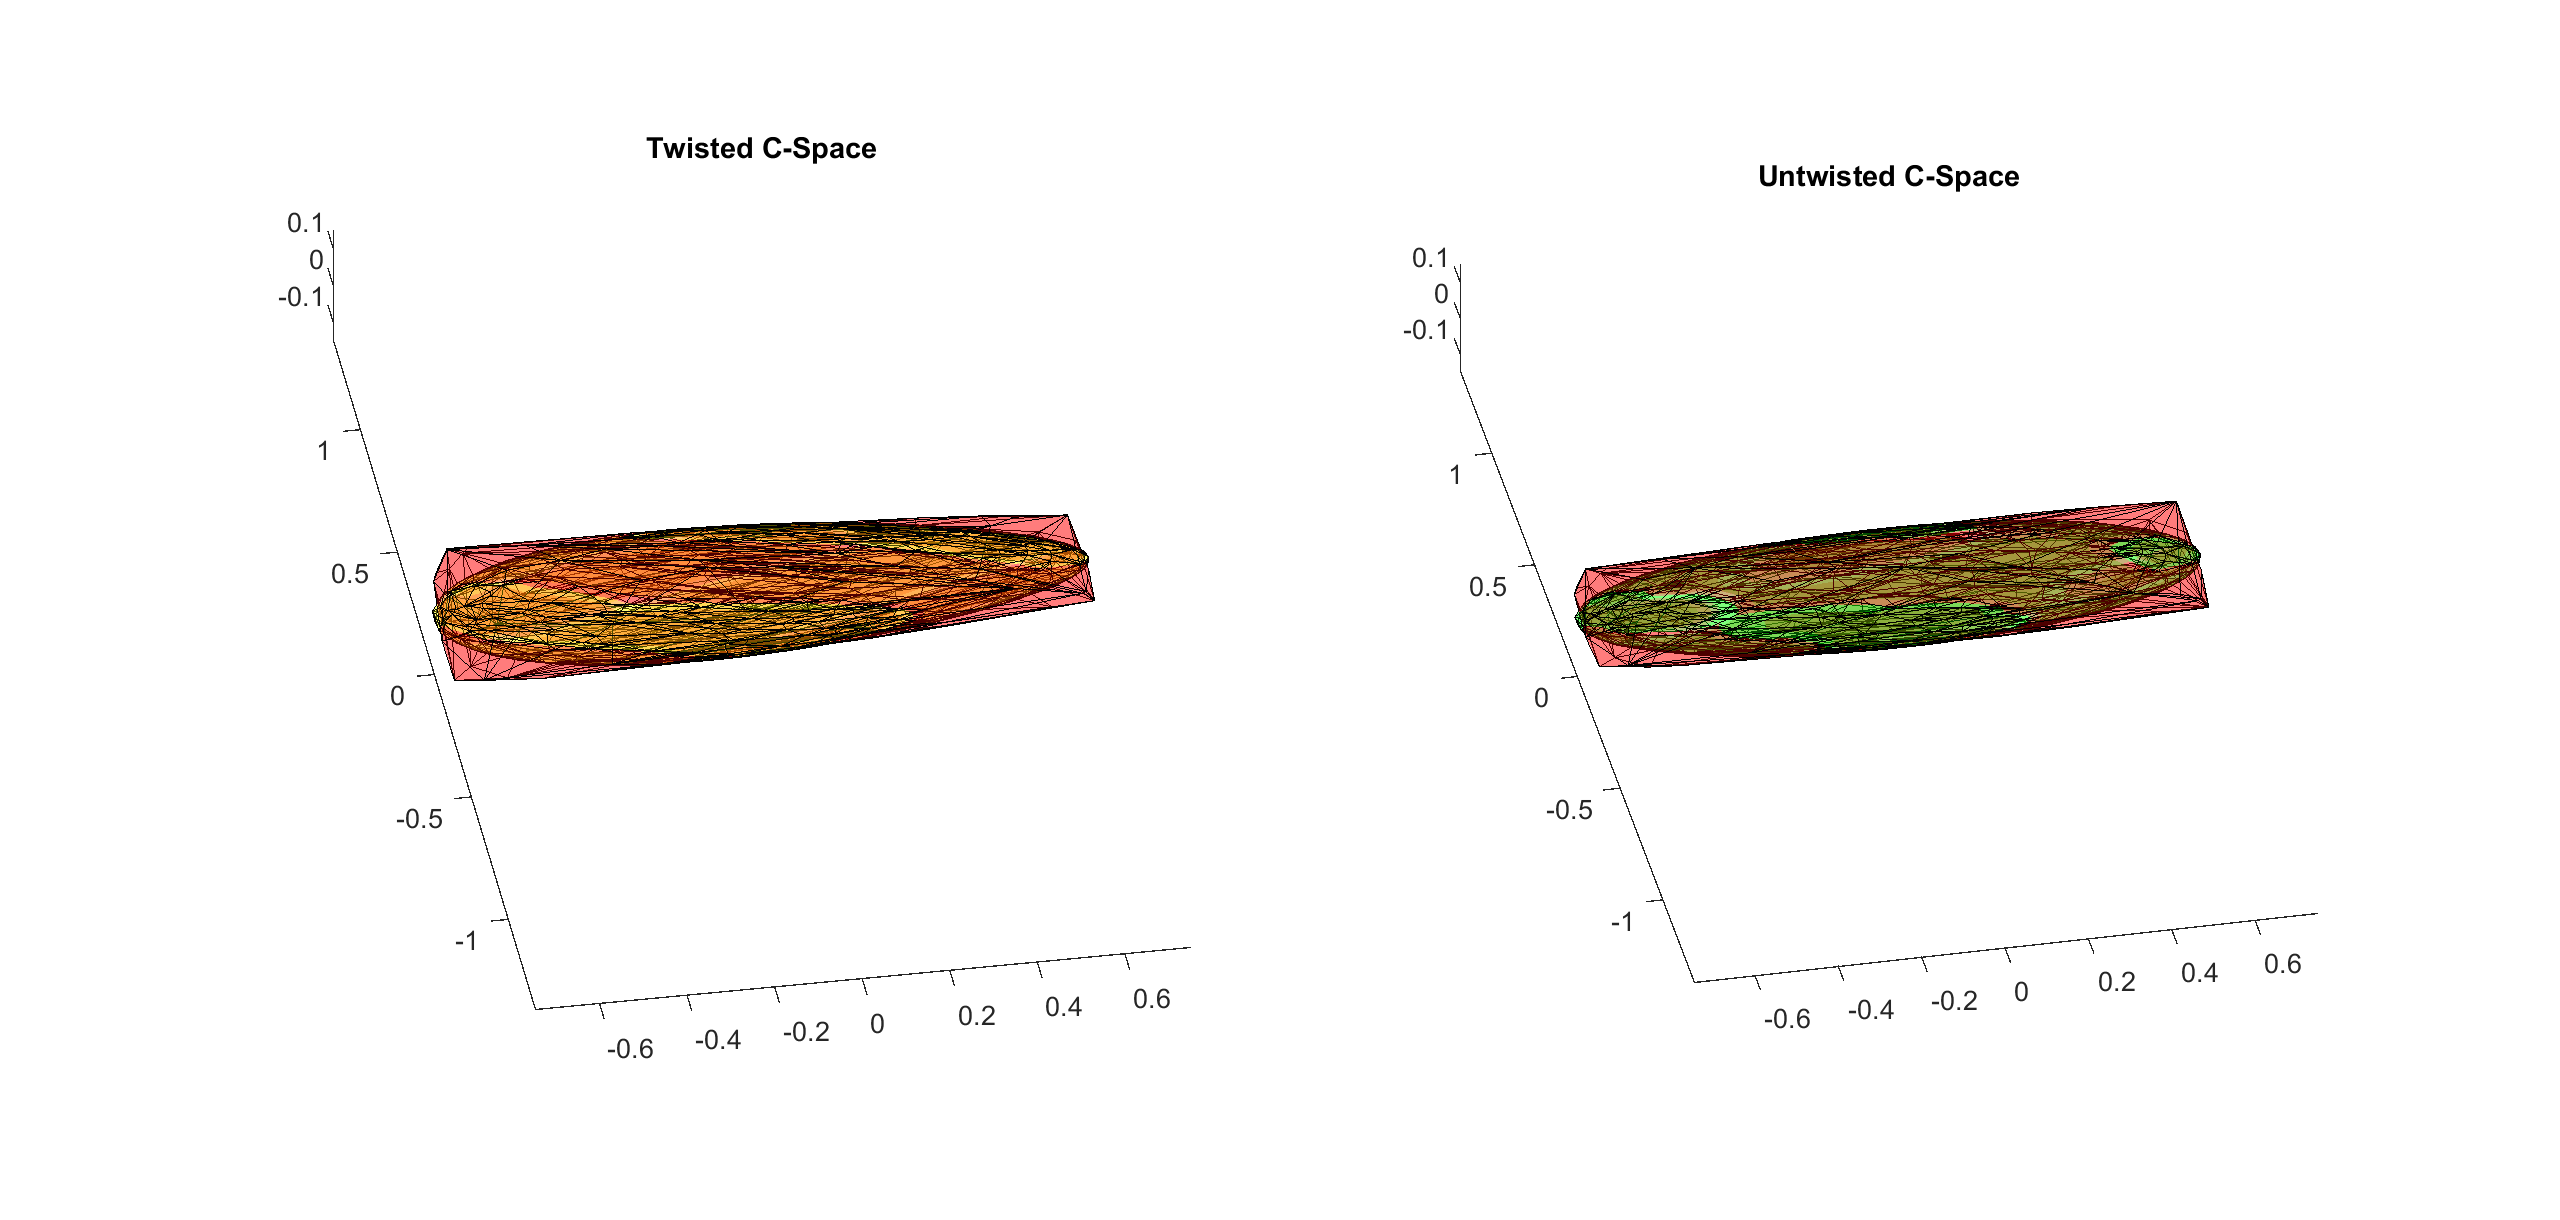
\includegraphics[scale = 0.25]{fig/twist-untwist_c-space_fit_scaled_ratio3.png}
\caption{heuristic fit, with parameters: $a_2 = 1.5$, $\alpha = 3$, $\epsilon = 0.1$, $\beta = 0.25x$, scale factor: 0.6}
\label{fit_scaled3}
\end{figure}

\item {\bf TODO list}
\begin{enumerate}
\item Find an automatic way to define the twisting function along x-axis, e.g. calculate the maximum ratio of $\theta/y$
\item Find a way to determine the scale factor of the heuristic fit inside the untwisted convex hull
\item Fit the untwisted convex hull with other shapes, e.g. superquadrics
\item Try the heuristic fit with different aspect ratios and explode factors
\end{enumerate}

\newpage
\item {\bf Heuristic KC with Polyhedron fit in C-Space, 2D}\\
Another observation from the sample-based KC is that surfaces between 3 different extreme points which seems flat forms a tetrahedron-shaped c-space. This gives an intuition to construct the motion c-space as a tetrahedron or generally a polyhedron. From this point, we first seek to find the extreme points that represent the polyhedron as follows.

\begin{enumerate}
\item {\bf Finding extreme vertices that represent the polyhedron}

Extreme points in $x$, $y$ and $\theta$ axes can be simply found by fixing the other two values to zero. For example, if we set $y,\theta = 0$, then the extreme distance in $x$-axis is $x_{extreme}=\epsilon a_1$; similarly $y_{extreme} = \epsilon a_2$ if fixing $x,\theta = 0$. The extreme distance in $\theta$-axis is obtained above in closed-form as $\theta_{extreme} = \arctan (\pm \epsilon \sqrt[]{\frac{\alpha}{(\alpha(1+\epsilon)-1)(\alpha - \epsilon - 1)}})$. Since in each axis, there are 2 extreme points (positive and negative), here we get 6 vertices for constructing the polyhedron.

Now we seek to find the vertices that are farthest to the origin. Let ${\bf z}=[\theta,x,y]^T$, then our goal is to maximize its distance function to origin, $f = {\bf z}^T {\bf z}$. Further, the constraint for ${\bf z}$ is that ${\bf t} = [x, y]^T$ and $\theta$ should satisfy the algebraic condition that the smaller ellipse $E_1$ must move inside the larger one $E_2$ without collision.
\begin{equation}
(R(\theta) \Lambda({\bf a}) {\bf u} + {\bf t})^T \Lambda^{-2}({\bf b}) (R(\theta) \Lambda({\bf a}) {\bf u} + {\bf t}) \leq 1
\end{equation}
Regrouping the terms of the first-order approximation of the above inequality gives the constraint for ${\bf z}$:
\begin{equation}
C({\bf z}) = {\bf z}^T H({\bf u}) {\bf z} + {\bf h}({\bf u})^T {\bf z} + c({\bf u}) \leq 1
\end{equation}

Such constraint is a family of inequality constraints where ${\bf u}_i = [\cos(\phi)_i, \sin(\phi)_i]^T$ represents the $i$-th point on the boundary of a unit circle. If we treat ${\bf z}$ as unknown variable and ${\bf u}$ as a group of known parameters, finding the maximum distance can be formed as an optimization problem as

\begin{equation}
\begin{aligned}
& {\bf z}_{extreme} = \arg\max {\bf z}^T {\bf z} \\
\text{{\bf s.t.   }} & C_i({\bf z}) = {\bf z}^T H({\bf u}_i) {\bf z} + {\bf h}({\bf u}_i)^T {\bf z} + c({\bf u}_i) \leq 1 & (i=0,...,n)\\
\end{aligned}
\end{equation}
where, $n$ is the number of discretized points on the boundary of the unit circle.

\begin{figure}[!b]
\centering
\begin{minipage}[b]{0.4\textwidth}
	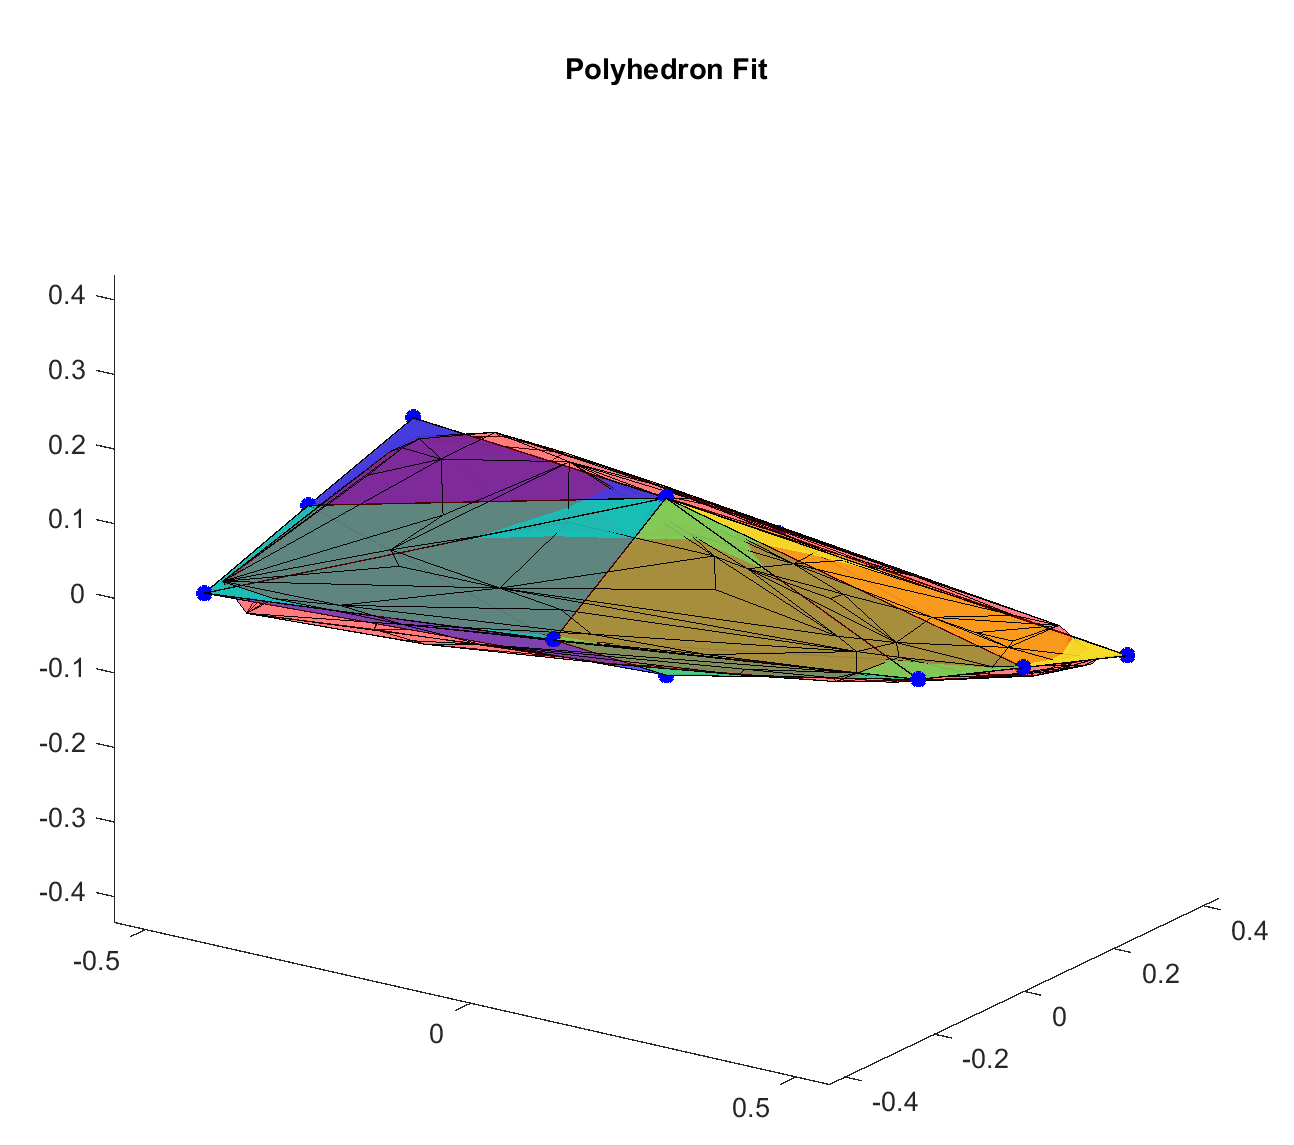
\includegraphics[scale = 0.2]{fig/c-space-polyhedron-fit.png}
	\caption{Heuristic fit as polyhedron represented by 10 extreme vertices, C-space}
	\label{polyfit_cspace}
\end{minipage}
\hfill
\begin{minipage}[b]{0.4\textwidth}
	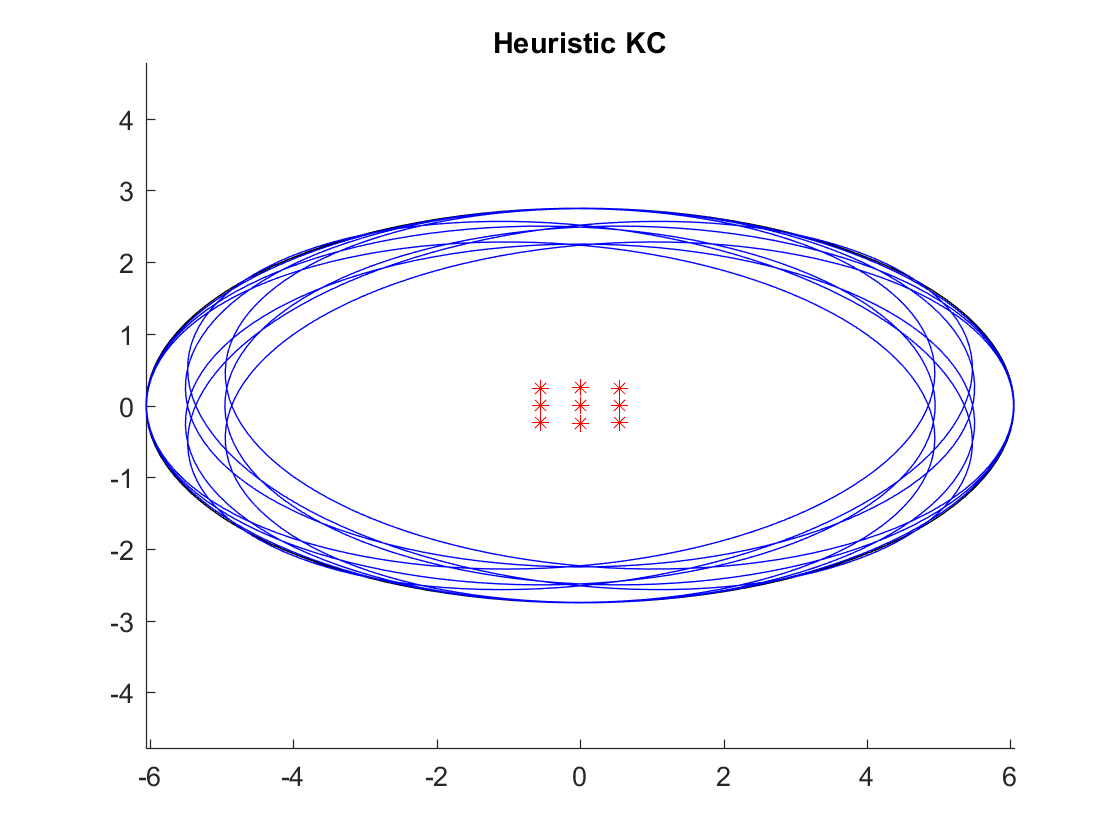
\includegraphics[scale = 0.25]{fig/ellipses-polyhedron-fit.png}
	\caption{Heuristic fit as polyhedron represented by 10 extreme vertices}
	\label{polyfit}
\end{minipage}
\end{figure}

Since the objective function is quadratic, the solutions for each variable have 2 possibilities, so the total number of solutions can be up to 8. However, not all of those possibilities are feasible solutions, meaning we have to validate them by substituting back to the constraint inequalities. Interestingly, after some numerical tests, there are only 4 of them that are feasible, i.e. for each fixed $x,y$ pair, there is only one corresponding $\theta$ that the smaller ellipse can stay inside the large one without collision. Fig \ref{polyfit_cspace} and \ref{polyfit} show the resulting c-space polyhedron and the corresponding scenarios in euclidean space.

At this time, we get totally 10 extreme vertices to construct the ``c-space motion polyhedron''. By saying ``polyhedron'', we should prove that the surfaces we observed is truly flat, in other word, points on the straight line connecting two vertices all represent safe configurations. This observation becomes obvious if we could firstly show that the constraint functions are convex.

\item {\bf Show that the c-space points inside the convex hull of the extreme vertices are safe configurations}\\
We have the following equivalent claim: the c-space points that lies on the line segment connecting any two extreme points also satisfy the conditions $C({\bf z}) = {\bf z}^T H({\bf u}) {\bf z} + {\bf h}({\bf u})^T {\bf z} + c({\bf u}) \leq 1$ for all ${\bf u} \in \mathcal{B}(1)$.

%%%% Proof of claim %%%%
\begin{proof}
From the condition we could also claim that among all ${\bf u}$,
\begin{equation}
\label{proof_convex}
\max C_i({\bf z}) = \max {\bf z}^T H({\bf u}_i) {\bf z} + {\bf h}({\bf u}_i)^T {\bf z} + c({\bf u}_i) \leq 1
\end{equation}

Then we could further prove that ``given any two extreme points ${\bf z}_1, {\bf z}_2$ satisfying \eqref{proof_convex}, the points on line segment between these two points also satisfy \eqref{proof_convex}''. The proof can be achieved by showing $\max C_i({\bf z})$ is convex.

For any fixed ${\bf u}_i$, we seek to prove, at first, that the function $C_i({\bf z})$ is convex, which is to show that, given ${\bf z}_1, {\bf z}_2$

\begin{equation}
\label{proof_convex_ineq}
C_i(\alpha {\bf z}_1 + (1-\alpha) {\bf z}_2) \leq \alpha C_i({\bf z}_1) + (1-\alpha) C_i({\bf z}_2),  \forall  \alpha \in [0,1]
\end{equation}

Expanding both sides and moving right-hand side to the left gives

\begin{equation}
\label{proof_convex_each}
\begin{aligned}
& [LHS]-[RHS] \\
=& [(\alpha {\bf z}_1 + (1-\alpha) {\bf z}_2)^T H({\bf u}_i) (\alpha {\bf z}_1 + (1-\alpha) {\bf z}_2) + {\bf h}({\bf u}_i)^T (\alpha {\bf z}_1 + (1-\alpha) {\bf z}_2) + c({\bf u}_i)]\\
& - [\alpha ({\bf z}_1^T H({\bf u}_i) {\bf z}_1 + {\bf h}({\bf u}_i)^T {\bf z}_1 + c({\bf u}_i)) + (1-\alpha)({\bf z}_2^T H({\bf u}_i) {\bf z}_2 + {\bf h}({\bf u}_i)^T {\bf z}_2 + c({\bf u}_i))] \\
=& -\alpha(1-\alpha) [({\bf z}_1 - {\bf z}_2)^T H({\bf u}_i) ({\bf z}_1 - {\bf z}_2)]
\end{aligned}
\end{equation}

The above expression satisfies the inequality $[LHS]-[RHS] \leq 0$ if and only if $({\bf z}_1 - {\bf z}_2)^T H({\bf u}_i) ({\bf z}_1 - {\bf z}_2) \geq 0$, or equivalently, $H({\bf u}_i)$ is symmetric positive semi-definite, which can be showed by expanding the original expression of the condition to the 1st-order approximation.

Since ${\bf z} = [{\bf r}^T, {\bf t}^T]^T$, only the quadratic terms with respect to both ${\bf r}$ and ${\bf t}$ from the 1st-order approximation will contribute to the calculation of ${\bf z}^T H({\bf u}_i) {\bf z}$ for any ${\bf z}$. Thus, we have, $\forall {\bf z} \in \mathfrak{R}^{\frac{n(n+1)}{2}}$

\begin{equation}
\label{proof_convex_psd}
{\bf z}^T H({\bf u}_i) {\bf z} = (S({\bf r}) \Lambda({\bf a}) {\bf u} + {\bf t})^T \Lambda^{-2}({\bf b}) (S({\bf r}) \Lambda({\bf a}) {\bf u} + {\bf t})
\end{equation}

Since $\Lambda^{-2}({\bf b})$ is diagonal with non-negative entries on diagonal, \eqref{proof_convex_psd} $\geq 0$, which means that $H({\bf u}_i)$ is symmetric positive semi-definite. Hence we showed the inequality condition for \eqref{proof_convex_each}, from which we conclude that each condition function $C_i({\bf z})$ is convex.

Next, we continue the proof by showing that the maximum of a family of convex functions is also convex. Since $C_i({\bf z})$ is convex, then taking maximum for both sides of \eqref{proof_convex_ineq} gives

\begin{equation}
\begin{aligned}
\max C_i(\alpha {\bf z}_1 + (1-\alpha) {\bf z}_2) &\leq \max [\alpha C_i({\bf z}_1) + (1-\alpha) C_i({\bf z}_2)],  \forall  \alpha \in [0,1]\\
&\leq \max \alpha C_i({\bf z}_1) + \max (1-\alpha) C_i({\bf z}_2),  \forall  \alpha \in [0,1] \\
\end{aligned}
\end{equation}

Thus $\max C_i({\bf z})$ is convex. And we can conclude that if for two extreme points ${\bf z}_1, {\bf z}_2$, $\max C_i({\bf z}_j) \leq 1, j=1,2$ are hold, then for points on the line segment between them, $\alpha {\bf z}_1 + (1-\alpha) {\bf z}_2, \forall \alpha \in [0,1]$, $\max C_i(\alpha {\bf z}_1 + (1-\alpha) {\bf z}_2) \leq \alpha \max C_i({\bf z}_1) + (1-\alpha) \max C_i({\bf z}_2) \leq 1$ is also satisfied. 
\end{proof}
%%%%%%%%%%%%

Figs \ref{polyfit_cspace_10000samples} and \ref{polyfit_10000samples} show the numerical results of randomly sampled configurations of smaller ellipses that verify the above claim. The ellipse whose configuration point is inside the c-space polyhedron (convex hull of the 10 extreme vertices) lies safely inside the larger one without collision.

\begin{figure}[t]
\centering
\begin{minipage}[b]{0.4\textwidth}
	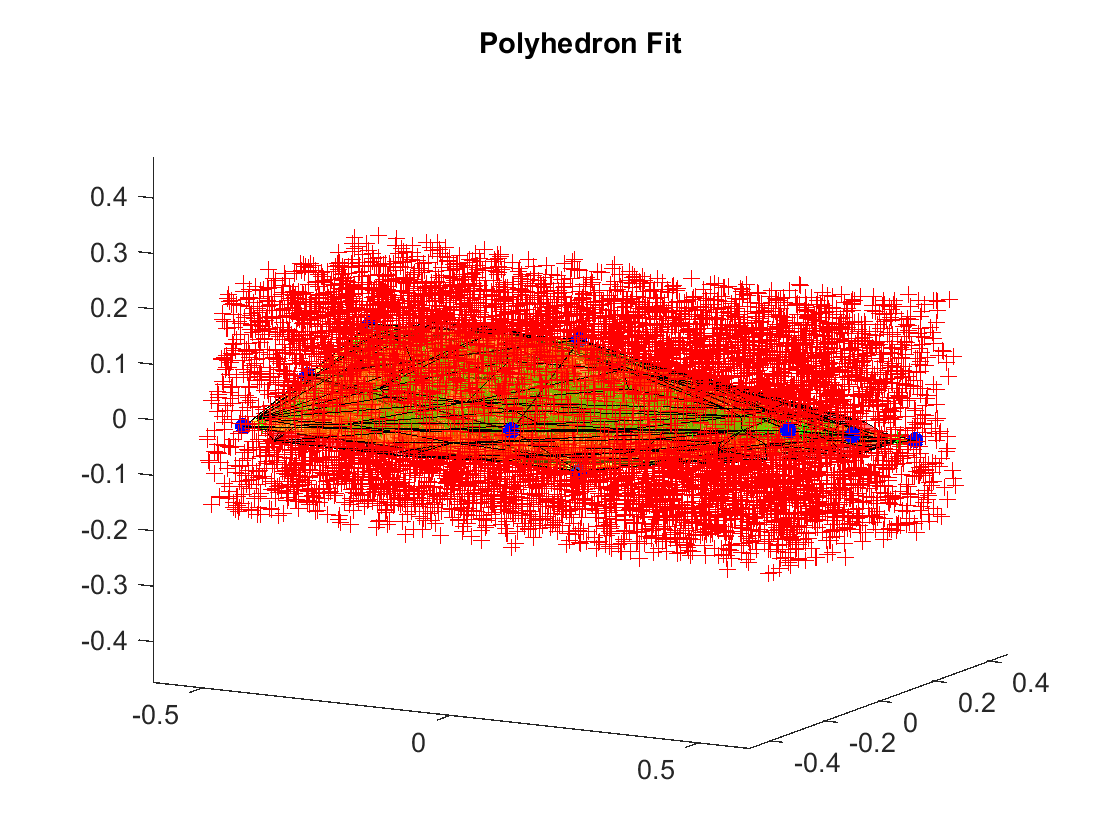
\includegraphics[scale = 0.2]{fig/c-space-polyhedron-fit-with-testPnts10000.png}
	\caption{C-space polyhedron fit with samples. Red: outside the convex hull; green: inside the convex hull}
	\label{polyfit_cspace_10000samples}
\end{minipage}
\hfill
\begin{minipage}[b]{0.4\textwidth}
	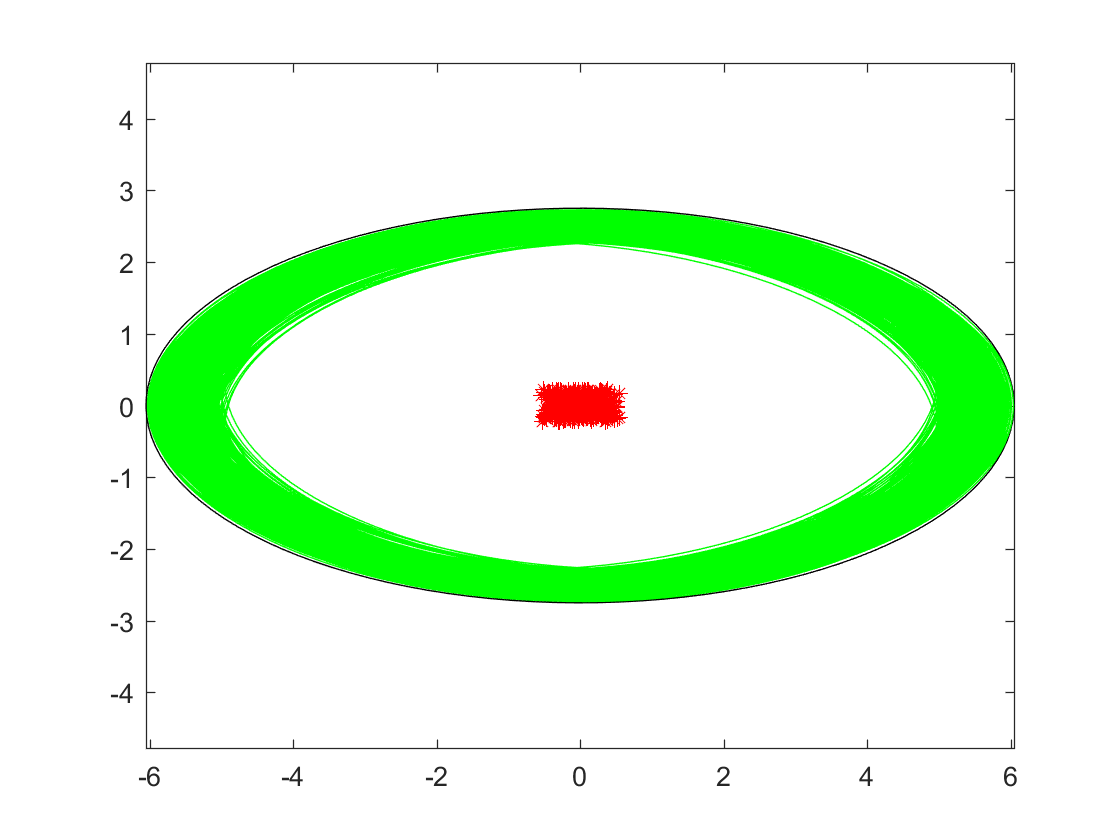
\includegraphics[scale = 0.25]{fig/ellipses-polyhedron-fit-with-testPnts10000.png}
	\caption{Smaller ellipses that lies safely inside the larger ellipse.}
	\label{polyfit_10000samples}
	\end{minipage}
\end{figure}

\end{enumerate}

\end{enumerate}
\end{document}
